\def\baselinestretch{1}
\chapter{Aplicaci\'on a datos de AFP}
\def\baselinestretch{1.0}
\goodbreak
\section{Introducci\'on}
En las siguientes secciones se introducir\'a algunos conceptos
del Sistema de Pensiones, se hablar\'a de su funci\'on, sus g\'enesis y la reforma de Previsi\'on
 Social.

Estos conceptos nos ayudar\'an para entender y analizar 7 AFP distintas en el p\'eriodo de Enero 1990-Febrero 2004
en su rentabilidad mensual.

Las AFP en Estudio son:
\begin{itemize}
\item 1 = AFP CUPRUM, 2 = AFP HABITAT, 3 = AFP PROVIDA, 4 = AFP PLANVITAL, 5\-=\-AFP STA MARIA, 6 = AFP SUMMA, 7 = AFP MAGISTER.
\end{itemize}

El ahorro de los trabajadores ha sido fundamental para el crecimiento y
desarrollo econ\'omico de Chile, ya que ha sido mayoritariamente invertido en
actividades productivas o crediticias haciendo posible el acceso a financiamiento
de miles de chilenos, sea para comprar la casa propia o acceder a productos a los
que nunca antes tuvo oportunidad.

El sistema de AFP ha operado en estos 26 a\~nos bajo el principio de Giro \'Unico
o exclusivo lo cual ha resguardado los fondos previsionales de problemas como
las ventas atadas y los conflictos de inter\'es, que surgen cuando un administrador
de ahorros distribuye conjuntamente otros productos y adem\'as gestiona
simult\'aneamente dineros propios y de terceros.

\section{Sistema de AFP}

En noviembre de 1980 se public\'o el D.L. 3.500 que estableci\'o un nuevo sistema de pensiones de Vejez, Invalidez y Sobrevivencia, sobre la base del ahorro de los trabajadores y la capitalizaci\'on en cuentas individuales.

El nuevo Sistema de Pensiones incorpora el concepto de propiedad de los ahorros previsionales por parte de los trabajadores afiliados, enfatizando la estrecha correspondencia entre el esfuerzo de ahorro realizado a lo largo de la vida activa de una persona y los beneficios en pensiones de vejez, invalidez y sobrevivencia que \'esta recibe.

As\'i tambi\'en, se instaura la administraci\'on de los ahorros por empresas privadas (AFP), con giro \'unico y con el rol de otorgar beneficios y prestaciones previsionales. La normativa que regula a estas instituciones, adem\'as de la ley, es dictada por la Superintendencia de AFP, la que adem\'as fiscaliza el adecuado funcionamiento de estas sociedades.

El objetivo del Sistema de Pensiones es proveer ingresos de reemplazo para los trabajadores que dejan la vida activa o laboral y cubrir los riesgos de invalidez (total o parcial) y de muerte del trabajador (sobrevivencia), de manera de proteger al afiliado y a su grupo familiar.

Se basa en el ahorro y la Capitalizaci\'on Individual. Los trabajadores dependientes cotizan obligatoriamente en las AFP y los independientes lo hacen en forma voluntaria. Los trabajadores son due\~nos de su ahorro previsional y en ellos recae la responsabilidad de preocuparse de su pensi\'on, sin perjuicio que el Estado garantice pensiones m\'inimas.

Otorga libertad de elecci\'on a los afiliados. De este modo el trabajador puede elegir la administradora que gestione sus ahorros previsionales y cambiarse cuando lo desee, as\'i como la edad a la que quiere pensionarse (jubilaci\'on por vejez o anticipada) y la modalidad de pago de pensi\'on (retiro programado, renta vitalicia o retiro programado con renta vitalicia diferida). Asimismo, puede elegir el Tipo de Fondo en donde invertir sus ahorros.

Es uniforme en la aplicaci\'on de las normas para todos los afiliados y establece directa relaci\'on entre las contribuciones de los trabajadores y los beneficios obtenidos.

La administraci\'on es privada y est\'a a cargo de sociedades an\'onimas especializadas.

\section{Rentabilidad de los Fondos de Pensiones}

La rentabilidad de los fondos es un factor determinante en un sistema de
capitalizaci\'on y ahorro individual, donde el saldo acumulado durante la vida
activa del trabajador incidir\'a significativamente en el monto de las pensiones.
De esta forma, un punto porcentual de mayor ganancia anual puede elevar el
monto de la pensi\'on al cabo de 30 \'o 40 a\~nos de ahorro entre un 25 $\%$ y 30 $\%$.
Tras 26 a\~nos del sistema de pensiones la rentabilidad promedio real anual
alcanza a UF $+ 10$ $\%$, un resultado muy superior al $4$ a $5$ $\%$ de la rentabilidad
estimada como suficiente para financiar pensiones de reemplazo con una tasa
del orden del $70$ $\%$ del promedio de las remuneraciones.

\section{Contribuci\'on al Desarrollo Econ\'omico}

Los fondos de pensiones han hecho un aporte significativo al desarrollo
econ\'omico de Chile, otorgando, asimismo, acceso a amplios sectores de la
poblaci\'on a servicios financieros a los que nunca hab\'ian podido acceder.
Para un pa\'is en desarrollo como Chile, hoy econom\'ia emergente, disponer de
ahorro fue siempre un problema y una aspiraci\'on, ya que es sabido que el
c\'irculo virtuoso del progreso comienza con el ahorro y sigue con la inversi\'on y
el crecimiento. En la actualidad un 25 $\%$ del total de activos financieros
nacionales pertenece a los fondos de pensiones de los trabajadores, lo cual
constituye un aporte tangible al desarrollo econ\'omico.

El mercado de capitales chileno se ha expandido en forma significativa los
\'ultimos 26 a\~nos, progreso en el cual el ahorro de los fondos de pensiones ha
jugado un rol clave. Se han convertido en una fuente de financiamiento para el
Estado, para los bancos y para las empresas. El sistema de pensiones ha
introducido competencia en el mercado de capitales.

Casi el 100 $\%$ del financiamiento de letras hipotecarias para la vivienda y bonos
de bancos pertenece a los fondos de pensiones; tambi\'en un 45 $\%$ de los bonos
de empresas y un 55 $\%$ de los t\'itulos estatales.

\section{Antiguo Sistema Previsional}

Chile fue el primer pa\'is de Am\'erica Latina que cre\'o un Sistema de Seguridad Social, a comienzos del siglo XX. A lo largo de los a\~{n}os se fueron creando diversos reg\'imenes de pensiones diferenciados por el tipo de actividad o grupos ocupacionales con reglas y beneficios distintos.

Es as\'i como llegan a coexistir 52 $"\mbox{Cajas}"$ o Instituciones de Previsi\'on que operaban bajo el esquema de reparto. Esto significa que los aportes de los afiliados activos financiaban las pensiones de los pasivos y, por tanto, la subsistencia del Sistema estaba supeditada a la relaci\'on trabajador/pensionado existente en la poblaci\'on en cada momento del tiempo.

Durante los primeros a\~nos de existencia del sistema, la proporci\'on de trabajadores fue suficiente para financiar los beneficios de los pensionados. Sin embargo, los cambios demogr\'aficos, que fueron reflejando una permanente disminuci\'on de la natalidad y un aumento en las expectativas de vida revirtieron esta relaci\'on, provocando un fuerte desfinanciamiento del Sistema.

Mientras que en el a\~no 1955, por cada 12,2 trabajadores cotizantes hab\'ia 1 pensionado, en 1980 por cada 2,5 trabajadores cotizantes hab\'ia 1 pensionado. Es decir, s\'olo en 25 a\~nos el costo de los trabajadores cotizantes, se increment\'o casi 5 veces.

Un agravante del problema del financiamiento lo constituy\'o la fuerte evasi\'on previsional, ya que a trabajadores y empleadores les resultaba m\'as econ\'omico hacer imposiciones por el m\'inimo legal, preocup\'andose s\'olo de imponer por valores reales los \'ultimos a\~{n}os de la vida activa del trabajador, cuando las imposiciones eran consideradas para la jubilaci\'on. Esta situaci\'on obligaba al Estado a elevar las imposiciones lo que, a su vez, incentivaba una mayor evasi\'on previsional y as\'i sucesivamente.

A ellos se agrega que el Estado fue proclive a otorgar beneficios sin el adecuado financiamiento, lo que acentu\'o el problema rese\~{n}ado, ocasionando un d\'eficit fiscal creciente, equivalente a un 28 $\%$ del gasto en la d\'ecada 1970 - 1980.\\
El Antiguo Sistema se caracteriz\'o tambi\'en por su falta de equidad. Dado que no exist\'ia una relaci\'on directa entre los aportes de los trabajadores y
los beneficios percibidos, se apreciaban notables desigualdades entre los m\'ultiples grupos cubiertos. Esta situaci\'on se sustentaba
en la facultad del poder pol\'itico para definir qui\'en se beneficiaba y cu\'anto, quedando de manifiesto el otorgamiento de mayores
concesiones a los grupos que ejerc\'ian mayor presi\'on. En efecto, en  el a\~no 1965 (1), los obreros chilenos, que representaban el 70
$\%$ de los cotizantes y cuyos ingresos eran los m\'as bajos, percib\'ian en t\'erminos absolutos, pensiones equivalentes a la mitad de lo que
obten\'ian los empleados privados y a 1/14 de lo obtenido por los empleados p\'ublicos, los cuales eran grupos de mayores ingresos. Al mismo tiempo,
el aporte efectuado por estos trabajadores en el mismo per\'iodo (2), era equivalente a m\'as del doble
del que realizaban los empleados p\'ublicos y s\'olo un 10 $\%$ inferior al de los privados.

Desde hac\'ia mucho tiempo en nuestro pa\'is se presentaba la necesidad de introducir cambios al sistema de Seguridad Social. Ya en la d\'ecada del '60 se elaboraron diversos informes sobre las falencias del antiguo sistema de Seguridad Social Chileno en los que se propon\'ian cambios profundos.

El desfinanciamiento y la inequidad del esquema de reparto dieron origen a una reforma Previsional que cre\'o, mediante el D.L. 3.500 de 1980, un Nuevo Sistema de Pensiones basado en la Capitalizaci\'on Individual y administrado por entidades privadas denominadas Administradoras de Fondos de Pensiones (AFP). El Antiguo Sistema continu\'o funcionando, principalmente a trav\'es de un ente \'unico, denominado Instituto de Normalizaci\'on Previsional (INP), el cual fusion\'o a las principales Cajas de Previsi\'on.

El Estado se hizo responsable del financiamiento de las cotizaciones pagadas en el Antiguo Sistema por aquellas personas que se cambiaron al Nuevo Sistema. Ello se materializa a trav\'es de unos instrumentos financieros denominados Bonos de Reconocimiento, los cuales son representativos de dichos per\'iodos de cotizaciones y que el trabajador hace efectivo al instante de pensionarse o fallecer.

El Bono de Reconocimiento se reajusta de acuerdo a la variaci\'on de la inflaci\'on y devenga un inter\'es del 4 $\%$ real anual, el cual se capitaliza cada a\~{n}o.

\section{Efecto Manada}

Uno de los vicios que se le han imputado al sistema de AFP es que si todas no invirtieran en
los mismos activos, quiz\'as inyectar\'ian competencia al mercado por la v\'ia de ofrecer mejores
 retornos a los afiliados.

Es por eso que las distintas AFP invierten en acciones en las mismas empresas, revelando que la rentabilidad en las distintas  AFP son similares.
Este fen\'omeno se llama Efecto Manada.

\subsection{Contexto y consecuencias de la competencia en rentabilidad v\'ia ranking}

Para entender el contexto de esta competencia, es \'util tener en mente dos hechos.
Primero, las magnitudes de las diferencias en rentabilidad tienden a ser peque\~nas. De hecho, 10 puntos base de mayor o menor rentabilidad pueden hacer la diferencia entre el primero y el \'ultimo en el ranking en un a\~no determinado.

Segundo, hay extrema transparencia en las decisiones de inversi\'on. Las carteras de todos los fondos de pensiones son conocidas 10 d\'ias despu\'es de cerrado el mes. Si se imagina que una buena decisi\'on de inversi\'on es una especie de invento, entonces, en este caso, no habr\'ia un per\'iodo de protecci\'on o patente de uso; todos podr\'ian conocerlo y utilizarlo en forma gratuita pocos d\'ias despu\'es de haber sido creado.

Lo anterior, en forma absolutamente natural, genera incentivos a situarse muy cerca del benchmark (o vara de medida), que en este caso es la cartera de la competencia relevante, y a tomar decisiones en el margen, relativamente peque\~nas en magnitud. N\'otese que la cantidad de trabajo o estudio necesarios para tomar una buena decisi\'on de inversi\'on es la misma, independientemente de la magnitud de la decisi\'on de inversi\'on tomada. El riesgo pertinente pasa a ser el comercial, que consiste en quedar en una mala posici\'on en el ranking de rentabilidad. Una medida que refleja adecuadamente que el riesgo se mide en t\'erminos relativos es el llamado tracking error o variabilidad de la diferencia de retorno con el sistema. El fen\'omeno descrito genera el llamado efecto manada o herding (lo que, en todo caso, no es exclusividad del sistema adoptado en Chile, ya que, se da en casi toda la industria de administraci\'on de carteras).

Algo que s\'i es particular del caso chileno es que existe por ley una rentabilidad m\'inima que se calcula con respecto al promedio del sistema de AFP. Esta norma tiende a reafirmar el comportamiento descrito en el p\'arrafo anterior, pero es probable que incluso sin rentabilidad m\'inima la forma de competir fuera similar.

\section{Acciones favoritas de las AFP}

Seg\'un Econsult, en un Articulo publicado el 8 de Abril de 2008, en el Diario La Tercera, revisado el Mi\'ercoles 23 de Julio 2008,16:45 hrs, mostr\'o que Provida, apuesta m\'as que el resto en CMPC, donde mantiene una sobreesposici\'on de 1.81$\%$ respecto de la Industria. Su segunda apuesta m\'as fuerte comparativamente hablando es Endesa y AntarChile. La segunda AFP por fondo administrativo, Habitat, tiene como favorita a Telef\'onica CTC, seguida por Endesa y AntarChile.

Planvital e ING Santa Mar\'ia,por ejemplo, favorecen m\'as a Soquimich que el sistema como un todo, aunque luego sus preferencias difieran. Cuprum, por su parte, favorece a Colb\'un, las acciones de Telef\'onica CTC y a Masisa; y al cierre de Junio Summa Bansander mostraba una mayor inclinaci\'on por Endesa, D$\&$S y Copec.
\subsection{El m\'etodo de Encosult}
Enconsult sum\'o la inversi\'on directa de cada AFP en acciones mantenidas en los fondos A, B, C, D y E. Con ello pudo determinar el porcentaje del fondo invertido en cada t\'itulo y observar cu\'ales son las acciones que m\'as pesan en el.

Luego la consultora tomo esa exposici\'on total del sistema en una acci\'on y le resto la exposici\'on particular de cada AFP. El calculo se efectu\'o excluyendo del total a cada administradora seg\'un fuera el caso (sistema sin Bansander, luego sin Provida y as\'i). De esta forma pudo determinar en que porcentaje cada administradora esta sobre o bajo la media exposici\'on del sistema para cada inversion, evitando la distorsi\'on de que la AFP se compare en cierto modo consigo misma


\section{An\'alisis Descriptivo}

En esta secci\'on se har\'a un sondeo, para entender como se han comportado las 7 AFP, desde un punto de vista descriptivo.
En esta primera parte se realizar\'a un conteo para saber cuantas veces han estado primeras, es decir, con la mayor rentabilidad, en el caso que una AFP tiene la mayor rentabilidad se le asignara un valor 1 y al resto de las AFP 0, entonces, finalmente se sumara todos los casos para saber cuantas veces estuvo primera en rentabilidad, si hay mas de un empate, es decir, que mas de dos AFP tienen la mayor rentabilidad, se le asignaran a cada una el valor 1.

La siguiente tabla muestra los resultados obtenidos, para las AFP en estudio.

\begin{small}
\begin{center}
\begin{tabular}{|l|l|ll}
\cline{1-2}
AFP & CONTEO &  &  \\
\cline{1-2}
Cuprum & 35 &  &  \\
Habitat & 38 &  &  \\
Magister & 44 &  &  \\
Planvital & 26 &  &  \\
Provida & 37 &  &  \\
Sta Maria & 21 &  &  \\
Summa & 38 &  &  \\
\cline{1-2}
\end{tabular}
\end{center}
\end{small}

Se observa que la AFP que estuvo con mayor rentabilidad y esta primera con 44 veces dentro de este conteo es la AFP Magister, seguido de la AFP Provida que estuvo 37 veces primera y la AFP Cuprum con 35 veces.

\begin{figure}[!htp]
\centering
\fbox{ 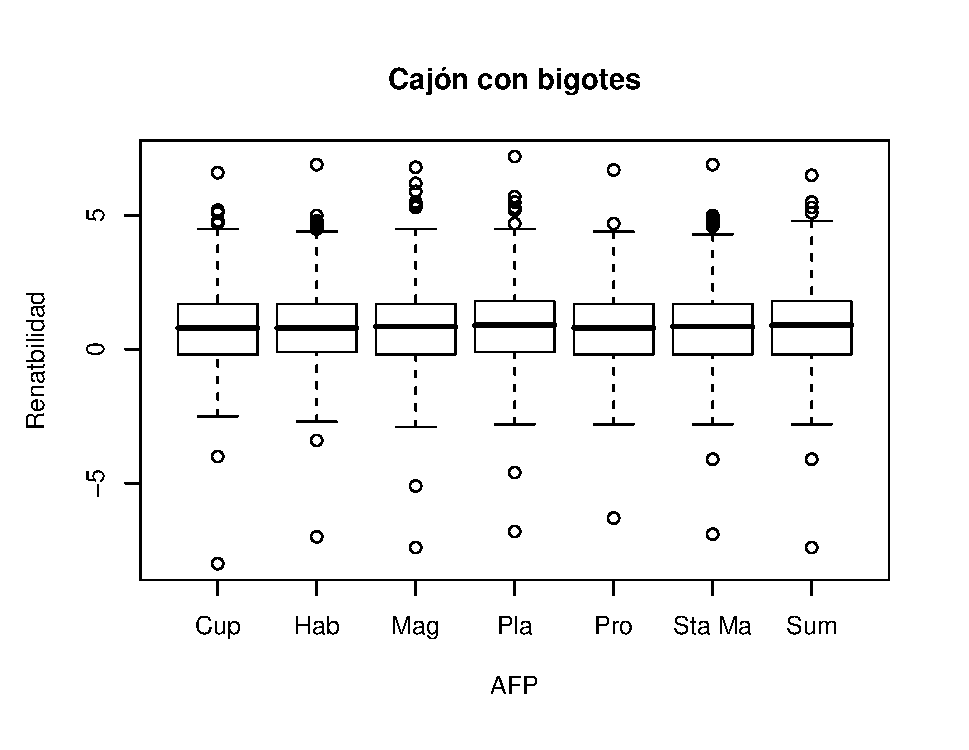
\includegraphics[height=4cm, width=6cm]{cajon.eps}}
\caption{Dispersi\'on de la rentabilidad de las AFP.}
\label{caja}
\end{figure}

Se puede observar que en gr\'afico de Caj\'on con bigotes, que hay datos que escapan a estos Cajones con bigotes. Adem\'as, las media son similares en todas las AFP. Acontinuaci\'on, se mostrara un sumario con algunas medidas descriptivas.


\begin{figure}[!htp]
\centering
\fbox{ 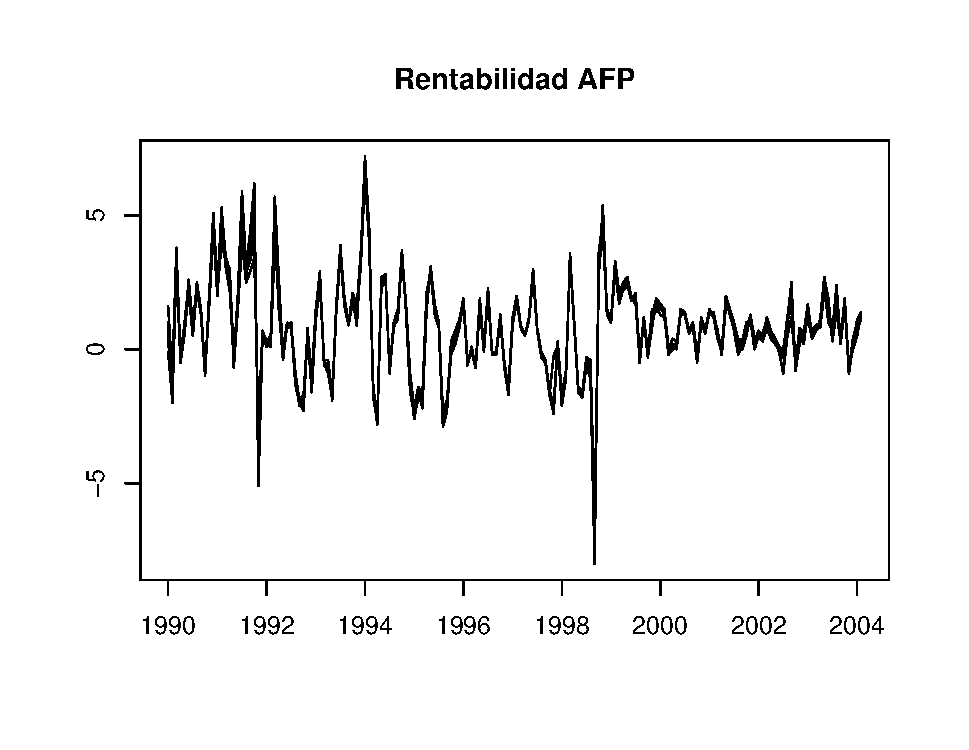
\includegraphics[height=4cm, width=6cm]{s_afp.eps}}
\caption{7 Series durante 1990 - 2004.}
\label{caja}
\end{figure}

En el siguiente gr\'afico se muestra el comportamiento de la rentabilidad en el tiempo de las 7 AFP, si se observa el gr\'afico se puede apreciar una linea gruesa, este fen\'omeno se denomina efecto manada el cual se ha mencionado anteriormente y en consecuencia no se puede notar grandes diferencias. En la siguiente tabla se muestra un an\'alisis descriptivo por AFP.

\begin{center}
\begin{small}
\begin{tabular}{|l|l|l|l|l|l|l|l|}
\hline
\multicolumn{1}{|c|}{Estad\'isticos} & \multicolumn{1}{c|}{Cuprum} & \multicolumn{1}{c|}{Habitat} & \multicolumn{1}{c|}{Magister} & \multicolumn{1}{c|}{Planvital} & \multicolumn{1}{c|}{Provida} & \multicolumn{1}{c|}{ING Sta Mar\'ia} & \multicolumn{1}{c|}{Summa} \\
\hline
\multicolumn{1}{|c|}{Media} & \multicolumn{1}{c|}{0,83} & \multicolumn{1}{c|}{0,82} & \multicolumn{1}{c|}{0,84} & \multicolumn{1}{c|}{0,86} & \multicolumn{1}{c|}{0,78} & \multicolumn{1}{c|}{0,80} & \multicolumn{1}{c|}{0,85} \\
\multicolumn{1}{|c|}{Mediana} & \multicolumn{1}{c|}{0,81} & \multicolumn{1}{c|}{0,83} & \multicolumn{1}{c|}{0,86} & \multicolumn{1}{c|}{0,90} & \multicolumn{1}{c|}{0,80} & \multicolumn{1}{c|}{0,87} & \multicolumn{1}{c|}{0,90} \\
\multicolumn{1}{|c|}{Moda} & \multicolumn{1}{c|}{-1,10} & \multicolumn{1}{c|}{0,80} & \multicolumn{1}{c|}{-1,70} & \multicolumn{1}{c|}{1,60} & \multicolumn{1}{c|}{-1,60} & \multicolumn{1}{c|}{0,90} & \multicolumn{1}{c|}{-1,70} \\
\multicolumn{1}{|c|}{Desv Est} & \multicolumn{1}{c|}{1,82} & \multicolumn{1}{c|}{1,77} & \multicolumn{1}{c|}{1,92} & \multicolumn{1}{c|}{1,88} & \multicolumn{1}{c|}{1,68} & \multicolumn{1}{c|}{1,80} & \multicolumn{1}{c|}{1,82} \\
\multicolumn{1}{|c|}{Varianza } & \multicolumn{1}{c|}{3,31} & \multicolumn{1}{c|}{3,12} & \multicolumn{1}{c|}{3,70} & \multicolumn{1}{c|}{3,53} & \multicolumn{1}{c|}{2,82} & \multicolumn{1}{c|}{3,24} & \multicolumn{1}{c|}{3,33} \\
\multicolumn{1}{|c|}{Coef Var} & \multicolumn{1}{c|}{220,07} & \multicolumn{1}{c|}{215,03} & \multicolumn{1}{c|}{230,05} & \multicolumn{1}{c|}{219,74} & \multicolumn{1}{c|}{215,82} & \multicolumn{1}{c|}{224,85} & \multicolumn{1}{c|}{214,81} \\
\multicolumn{1}{|c|}{Rango} & \multicolumn{1}{c|}{14,60} & \multicolumn{1}{c|}{13,90} & \multicolumn{1}{c|}{14,20} & \multicolumn{1}{c|}{14,00} & \multicolumn{1}{c|}{13,00} & \multicolumn{1}{c|}{13,80} & \multicolumn{1}{c|}{13,90} \\
\multicolumn{1}{|c|}{M\'inimo} & \multicolumn{1}{c|}{-8,00} & \multicolumn{1}{c|}{-7,00} & \multicolumn{1}{c|}{-7,40} & \multicolumn{1}{c|}{-6,80} & \multicolumn{1}{c|}{-6,30} & \multicolumn{1}{c|}{-6,90} & \multicolumn{1}{c|}{-7,40} \\
\multicolumn{1}{|c|}{M\'aximo} & \multicolumn{1}{c|}{6,60} & \multicolumn{1}{c|}{6,90} & \multicolumn{1}{c|}{6,80} & \multicolumn{1}{c|}{7,20} & \multicolumn{1}{c|}{6,70} & \multicolumn{1}{c|}{6,90} & \multicolumn{1}{c|}{6,50} \\
\multicolumn{1}{|c|}{Cuenta} & \multicolumn{1}{c|}{170,00} & \multicolumn{1}{c|}{170,00} & \multicolumn{1}{c|}{170,00} & \multicolumn{1}{c|}{170,00} & \multicolumn{1}{c|}{170,00} & \multicolumn{1}{c|}{170,00} & \multicolumn{1}{c|}{170,00} \\
\hline
\end{tabular}
\end{small}
\end{center}

Si se observa la tabla se puede destacar que la rentabilidad media de Cuprum es de 0.8265, las rentabilidades extremas se pueden apreciar con un m\'inimo de -6.3 y un m\'aximo de 6.7. Adem\'as, se puede apreciar que en un 25$\%$ la rentabilidad llega a -0.175 y en el 75$\%$ llega a 1.7. Es claro, mencionar que para el resto de las AFP la interpretaci\'on es la misma.

M\'as adelante se estudiar\'an estas AFP, para representar, a trav\'es, de modelos param\'etricos y ver cual modelo puede representar mejor esta situaci\'on.

\section{Aplicaci\'on \'Indice de Comovimiento o Codispersi\'on}

Para el conjunto de 7 AFP, se calculara el \'Indice de Comovimiento para determinar en que grado comueven, los resultados son:

\paragraph{\'Indice de Comovimiento con $h=1$.}
\begin{center}
\begin{small}
\begin{tabular}{|l|l|l|l|l|l|l|lllllll}
\cline{1-7}
\multicolumn{1}{|c|}{$\rho(h=1)$} & \multicolumn{1}{c|}{Cuprum} & \multicolumn{1}{c|}{Habitat} & \multicolumn{1}{c|}{Provida} & \multicolumn{1}{c|}{Planvital} & \multicolumn{1}{c|}{Sta Mar\'ia} & \multicolumn{1}{c|}{Summa} &  &  &  &  &  &  &  \\
\cline{1-7}
\multicolumn{1}{|c|}{Habitat} & \multicolumn{1}{c|}{0,990} & \multicolumn{1}{c|}{} & \multicolumn{1}{c|}{} & \multicolumn{1}{c|}{} & \multicolumn{1}{c|}{} & \multicolumn{1}{c|}{} &  &  &  &  &  &  &  \\
\cline{1-7}
\multicolumn{1}{|c|}{Provida} & \multicolumn{1}{c|}{0,984} & \multicolumn{1}{c|}{0,982} & \multicolumn{1}{c|}{} & \multicolumn{1}{c|}{} & \multicolumn{1}{c|}{} & \multicolumn{1}{c|}{} &  &  &  &  &  &  &  \\
\cline{1-7}
\multicolumn{1}{|c|}{Planvital} & \multicolumn{1}{c|}{0,983} & \multicolumn{1}{c|}{0,987} & \multicolumn{1}{c|}{0,993} & \multicolumn{1}{c|}{} & \multicolumn{1}{c|}{} & \multicolumn{1}{c|}{} &  &  &  &  &  &  &  \\
\cline{1-7}
\multicolumn{1}{|c|}{Sta Maria} & \multicolumn{1}{c|}{0,982} & \multicolumn{1}{c|}{0,993} & \multicolumn{1}{c|}{0,970} & \multicolumn{1}{c|}{0,979} & \multicolumn{1}{c|}{} & \multicolumn{1}{c|}{} &  &  &  &  &  &  &  \\
\cline{1-7}
\multicolumn{1}{|c|}{Summa} & \multicolumn{1}{c|}{0,991} & \multicolumn{1}{c|}{0,995} & \multicolumn{1}{c|}{0,988} & \multicolumn{1}{c|}{0,992} & \multicolumn{1}{c|}{0,989} & \multicolumn{1}{c|}{} &  &  &  &  &  &  &  \\
\cline{1-7}
\multicolumn{1}{|c|}{Magister} & \multicolumn{1}{c|}{0,986} & \multicolumn{1}{c|}{0,985} & \multicolumn{1}{c|}{0,983} & \multicolumn{1}{c|}{0,986} & \multicolumn{1}{c|}{0,975} & \multicolumn{1}{c|}{0,987} &  &  &  &  &  &  &  \\
\cline{1-7}
\end{tabular}
\end{small}
\end{center}

Se puede observar que el comovimiento  entre las AFP es similar, es decir, estas comueven casi perfectamente en cualquier instante de tiempo.

\paragraph{\'Indice de Comovimiento con $h=2$.}

De igual forma si se calcula ahora con $h=2$, se puede apreciar los siguientes resultados:

\begin{center}
\begin{small}
\begin{tabular}{|l|l|l|l|l|l|l|lllllll}
\cline{1-7}
\multicolumn{1}{|c|}{$\rho(h=2)$} & \multicolumn{1}{c|}{Cuprum} & \multicolumn{1}{c|}{Habitat} & \multicolumn{1}{c|}{Provida} & \multicolumn{1}{c|}{Planvital} & \multicolumn{1}{c|}{Sta Mar\'ia} & \multicolumn{1}{c|}{Summa} &  &  &  &  &  &  &  \\
\cline{1-7}
\multicolumn{1}{|c|}{Habitat} & \multicolumn{1}{c|}{0,990} & \multicolumn{1}{c|}{} & \multicolumn{1}{c|}{} & \multicolumn{1}{c|}{} & \multicolumn{1}{c|}{} & \multicolumn{1}{c|}{} &  &  &  &  &  &  &  \\
\cline{1-7}
\multicolumn{1}{|c|}{Provida} & \multicolumn{1}{c|}{0,987} & \multicolumn{1}{c|}{0,985} & \multicolumn{1}{c|}{} & \multicolumn{1}{c|}{} & \multicolumn{1}{c|}{} & \multicolumn{1}{c|}{} &  &  &  &  &  &  &  \\
\cline{1-7}
\multicolumn{1}{|c|}{Planvital} & \multicolumn{1}{c|}{0,989} & \multicolumn{1}{c|}{0,987} & \multicolumn{1}{c|}{0,993} & \multicolumn{1}{c|}{} & \multicolumn{1}{c|}{} & \multicolumn{1}{c|}{} &  &  &  &  &  &  &  \\
\cline{1-7}
\multicolumn{1}{|c|}{Sta Maria} & \multicolumn{1}{c|}{0,983} & \multicolumn{1}{c|}{0,994} & \multicolumn{1}{c|}{0,970} & \multicolumn{1}{c|}{0,979} & \multicolumn{1}{c|}{} & \multicolumn{1}{c|}{} &  &  &  &  &  &  &  \\
\cline{1-7}
\multicolumn{1}{|c|}{Summa} & \multicolumn{1}{c|}{0,992} & \multicolumn{1}{c|}{0,995} & \multicolumn{1}{c|}{0,988} & \multicolumn{1}{c|}{0,992} & \multicolumn{1}{c|}{0,989} & \multicolumn{1}{c|}{} &  &  &  &  &  &  &  \\
\cline{1-7}
\multicolumn{1}{|c|}{Magister} & \multicolumn{1}{c|}{0,990} & \multicolumn{1}{c|}{0,985} & \multicolumn{1}{c|}{0,983} & \multicolumn{1}{c|}{0,986} & \multicolumn{1}{c|}{0,975} & \multicolumn{1}{c|}{0,987} &  &  &  &  &  &  &  \\
\cline{1-7}
\end{tabular}
\end{small}
\end{center}

Los valores est\'an cercanos a $1$, es decir, que las series se mueven conjuntamente iguales en cualquier periodo de tiempo $[t_i,t_{i+2}]$ En este caso los valores son similares a la tabla anterior.

\paragraph{\'Indice de Comovimiento con $h=3$.}

Ahora con $h=3$, se pueden apreciar valores similares.

\begin{center}
\begin{small}
\begin{tabular}{|l|l|l|l|l|l|l|lllllll}
\cline{1-7}
\multicolumn{1}{|c|}{$\rho(h=3)$} & \multicolumn{1}{c|}{Cuprum} & \multicolumn{1}{c|}{Habitat} & \multicolumn{1}{c|}{Provida} & \multicolumn{1}{c|}{Planvital} & \multicolumn{1}{c|}{Sta Mar\'ia} & \multicolumn{1}{c|}{Summa} &  &  &  &  &  &  &  \\
\cline{1-7}
\multicolumn{1}{|c|}{Habitat} & \multicolumn{1}{c|}{0,988} & \multicolumn{1}{c|}{} & \multicolumn{1}{c|}{} & \multicolumn{1}{c|}{} & \multicolumn{1}{c|}{} & \multicolumn{1}{c|}{} &  &  &  &  &  &  &  \\
\cline{1-7}
\multicolumn{1}{|c|}{Provida} & \multicolumn{1}{c|}{0,986} & \multicolumn{1}{c|}{0,987} & \multicolumn{1}{c|}{} & \multicolumn{1}{c|}{} & \multicolumn{1}{c|}{} & \multicolumn{1}{c|}{} &  &  &  &  &  &  &  \\
\cline{1-7}
\multicolumn{1}{|c|}{Planvital} & \multicolumn{1}{c|}{0,988} & \multicolumn{1}{c|}{0,987} & \multicolumn{1}{c|}{0,993} & \multicolumn{1}{c|}{} & \multicolumn{1}{c|}{} & \multicolumn{1}{c|}{} &  &  &  &  &  &  &  \\
\cline{1-7}
\multicolumn{1}{|c|}{Sta Maria} & \multicolumn{1}{c|}{0,981} & \multicolumn{1}{c|}{0,994} & \multicolumn{1}{c|}{0,970} & \multicolumn{1}{c|}{0,979} & \multicolumn{1}{c|}{} & \multicolumn{1}{c|}{} &  &  &  &  &  &  &  \\
\cline{1-7}
\multicolumn{1}{|c|}{Summa} & \multicolumn{1}{c|}{0,990} & \multicolumn{1}{c|}{0,995} & \multicolumn{1}{c|}{0,988} & \multicolumn{1}{c|}{0,992} & \multicolumn{1}{c|}{0,989} & \multicolumn{1}{c|}{} &  &  &  &  &  &  &  \\
\cline{1-7}
\multicolumn{1}{|c|}{Magister} & \multicolumn{1}{c|}{0,983} & \multicolumn{1}{c|}{0,985} & \multicolumn{1}{c|}{0,983} & \multicolumn{1}{c|}{0,986} & \multicolumn{1}{c|}{0,975} & \multicolumn{1}{c|}{0,987} &  &  &  &  &  &  &  \\
\cline{1-7}
\end{tabular}
\end{small}
\end{center}

\paragraph{\'Indice de Comovimiento con $h=4$.}

 Finalmente con $h=4$, las diferencias entre valores no son significativa por simple inspecci\'on.

\begin{center}
\begin{small}
\begin{tabular}{|l|l|l|l|l|l|l|lllllll}
\cline{1-7}
\multicolumn{1}{|c|}{$\rho(h=4)$} & \multicolumn{1}{c|}{Cuprum} & \multicolumn{1}{c|}{Habitat} & \multicolumn{1}{c|}{Provida} & \multicolumn{1}{c|}{Planvital} & \multicolumn{1}{c|}{Sta Mar\'ia} & \multicolumn{1}{c|}{Summa} &  &  &  &  &  &  &  \\
\cline{1-7}
\multicolumn{1}{|c|}{Habitat} & \multicolumn{1}{c|}{0,990} & \multicolumn{1}{c|}{} & \multicolumn{1}{c|}{} & \multicolumn{1}{c|}{} & \multicolumn{1}{c|}{} & \multicolumn{1}{c|}{} &  &  &  &  &  &  &  \\
\cline{1-7}
\multicolumn{1}{|c|}{Provida} & \multicolumn{1}{c|}{0,986} & \multicolumn{1}{c|}{0,987} & \multicolumn{1}{c|}{} & \multicolumn{1}{c|}{} & \multicolumn{1}{c|}{} & \multicolumn{1}{c|}{} &  &  &  &  &  &  &  \\
\cline{1-7}
\multicolumn{1}{|c|}{Planvital} & \multicolumn{1}{c|}{0,989} & \multicolumn{1}{c|}{0,989} & \multicolumn{1}{c|}{0,993} & \multicolumn{1}{c|}{} & \multicolumn{1}{c|}{} & \multicolumn{1}{c|}{} &  &  &  &  &  &  &  \\
\cline{1-7}
\multicolumn{1}{|c|}{Sta Maria} & \multicolumn{1}{c|}{0,982} & \multicolumn{1}{c|}{0,993} & \multicolumn{1}{c|}{0,970} & \multicolumn{1}{c|}{0,979} & \multicolumn{1}{c|}{} & \multicolumn{1}{c|}{} &  &  &  &  &  &  &  \\
\cline{1-7}
\multicolumn{1}{|c|}{Summa} & \multicolumn{1}{c|}{0,992} & \multicolumn{1}{c|}{0,995} & \multicolumn{1}{c|}{0,988} & \multicolumn{1}{c|}{0,992} & \multicolumn{1}{c|}{0,989} & \multicolumn{1}{c|}{} &  &  &  &  &  &  &  \\
\cline{1-7}
\multicolumn{1}{|c|}{Magister} & \multicolumn{1}{c|}{0,990} & \multicolumn{1}{c|}{0,985} & \multicolumn{1}{c|}{0,983} & \multicolumn{1}{c|}{0,986} & \multicolumn{1}{c|}{0,975} & \multicolumn{1}{c|}{0,987} &  &  &  &  &  &  &  \\
\cline{1-7}
\end{tabular}
\end{small}
\end{center}

Este alto grado de comovimiento, se puede deber a que las AFP bajo el fen\'omeno de efecto manada, comuevan casi perfectamente en cualquier instante de tiempo $[t_i,t_{i+h}]$.

\section{Modelamiento}

Como se mencion\'o anteriormente, se estudiar\'a la estacionariedad y el comportamiento de la rentabilidad. Para poder modelar esta situaci\'on se usar\'a las definiciones de series de tiempo mencionadas anteriormente y se estudiara como se comportan respecto al \'indice o coeficiente de Codispersi\'on para ver cual es su grado de comovimiento.

Por otra parte, se aplicar\'a el \'indice de disimilaridad, para clasificar las AFP respecto a su rentabilidad y considerando la estructura de correlaci\'on temporal, esto ayudar\'a a responder los objetivos de este Proyecto de T\'itulo.

Las hip\'otesis que contempla este Proyecto de T\'itulo, es que las series que se estudiaran son estacionarias.

Para analizar la estacionalidad, hay varios aspectos que se tienen que considerar, proponer transformaciones que ayudar\'an a estabilizar la varianza unas propuestas son $\log{x}$, $\sqrt{x}$, $\frac{1}{x}$ y desplazar la serie en $c$ por nombrar algunas. Otra alternativa es, a trav\'es, de la estructura de correlaci\'on temporal que en este caso es la funci\'on de autocorrelaci\'on (ACF) y funci\'on de autocorrelaci\'on parcial (Partial ACF), estas estructuras ayudaran a proponer un modelo que se pueda ajustar mejor a esta situaci\'on.

Para esto, existen valores que nos ayudan a comparar cuales de los modelos se ajusta mejor, como es el criterio Akaike (AIC), donde el AIC m\'as peque\~{n}o evidencia un mejor ajuste. Observando las series por separado, como muestra la siguiente figura.


\begin{figure}[!ht]
\begin{center}
\centering
  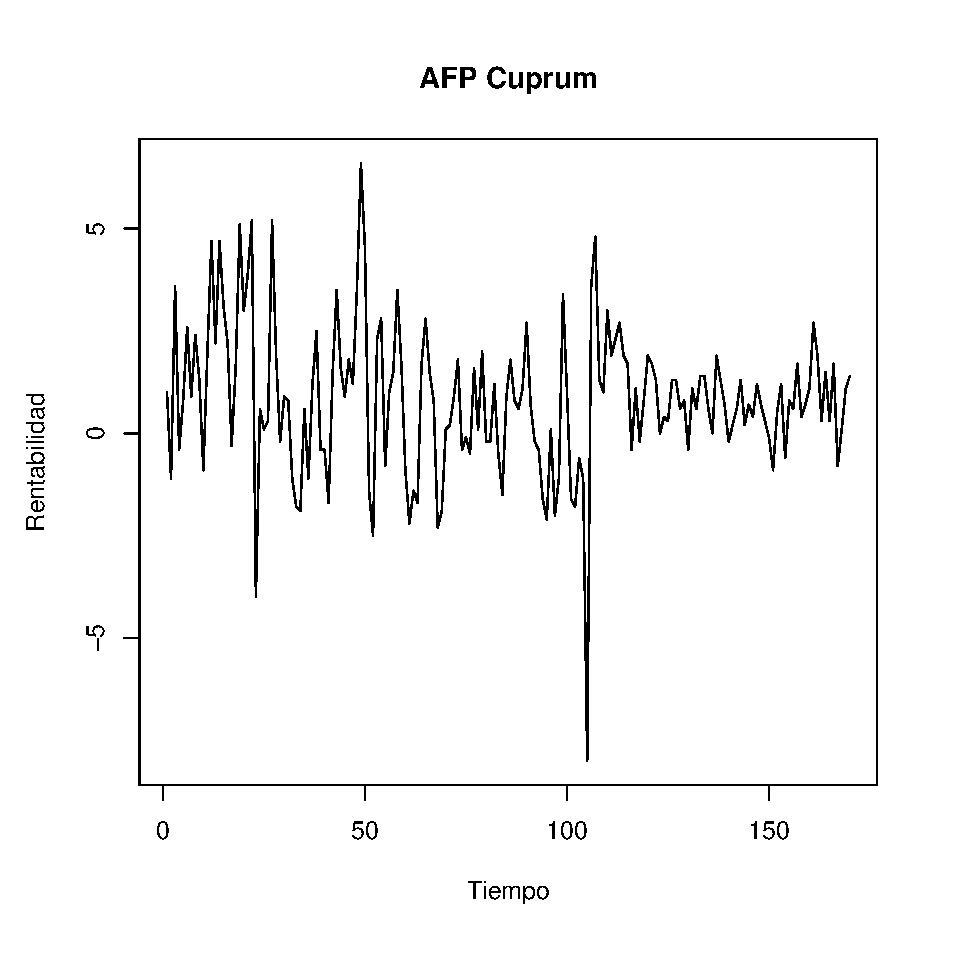
\includegraphics[height=4cm, width=4cm]{afp1.eps}
  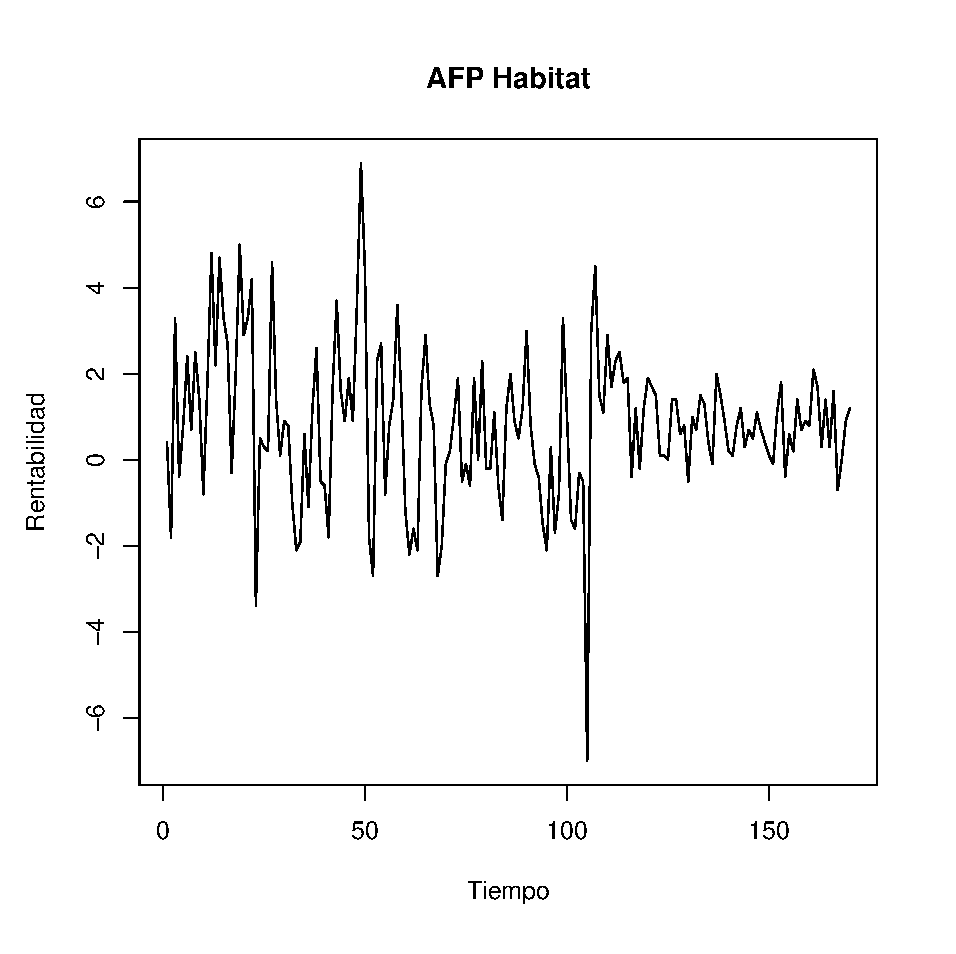
\includegraphics[height=4cm, width=4cm]{afp2.eps}
  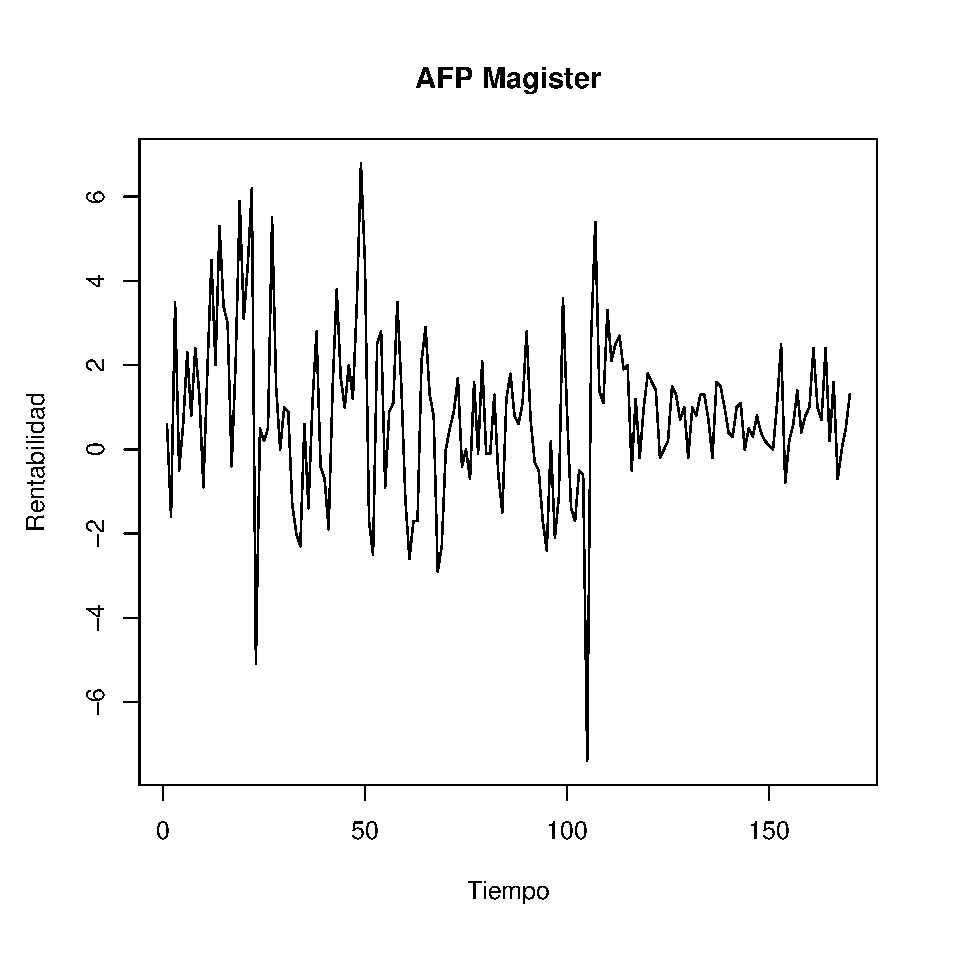
\includegraphics[height=4cm, width=4cm]{afp3.eps}
  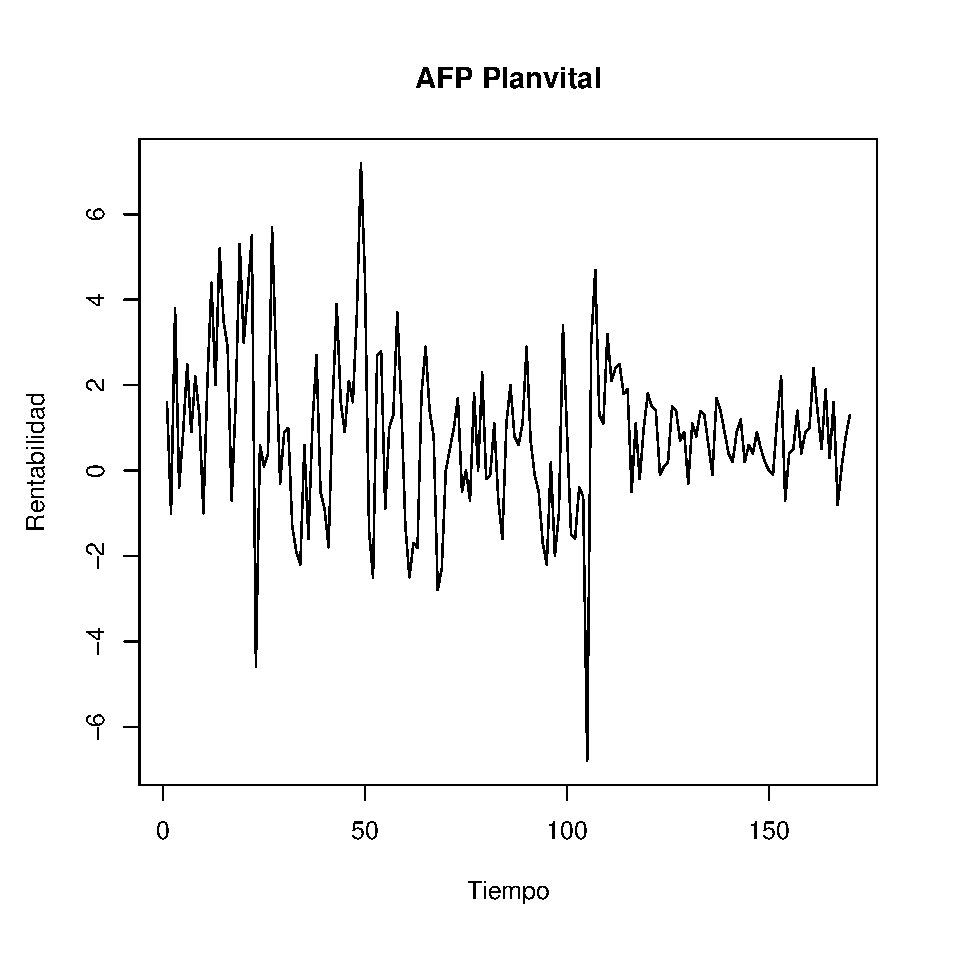
\includegraphics[height=4cm, width=4cm]{afp4.eps}\\
  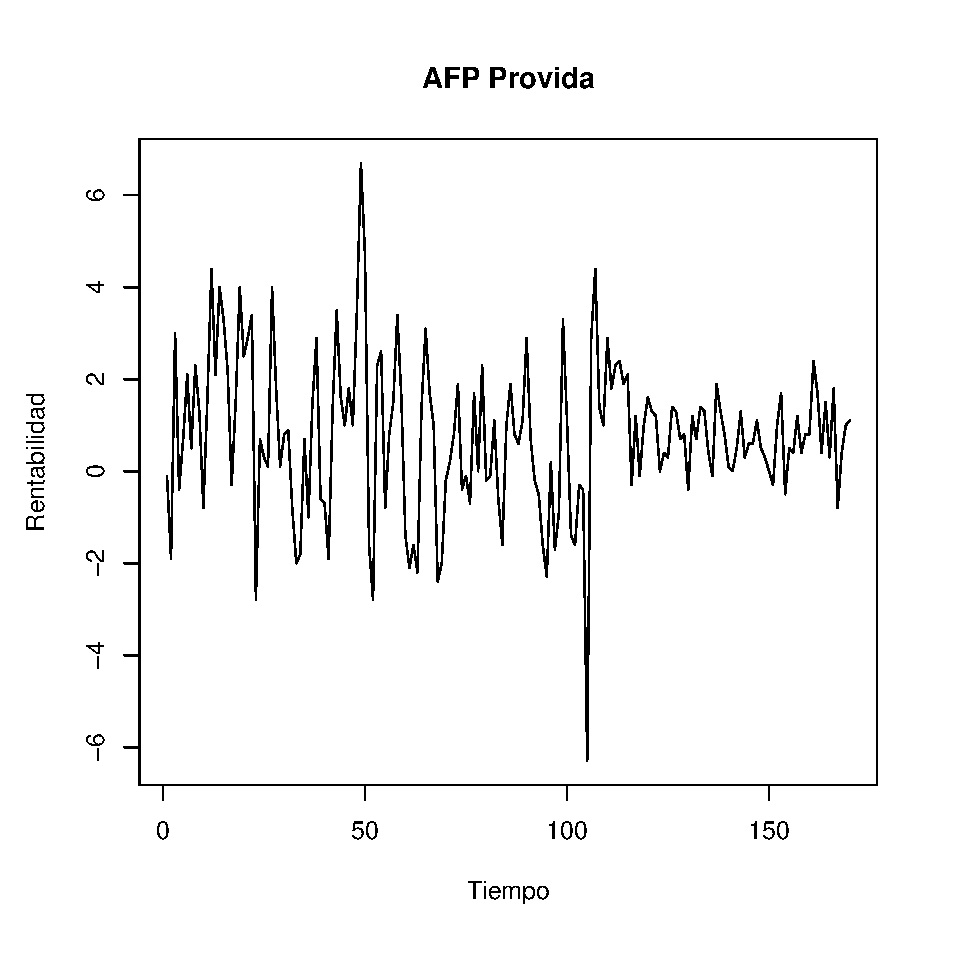
\includegraphics[height=4cm, width=4cm]{afp5.eps}
  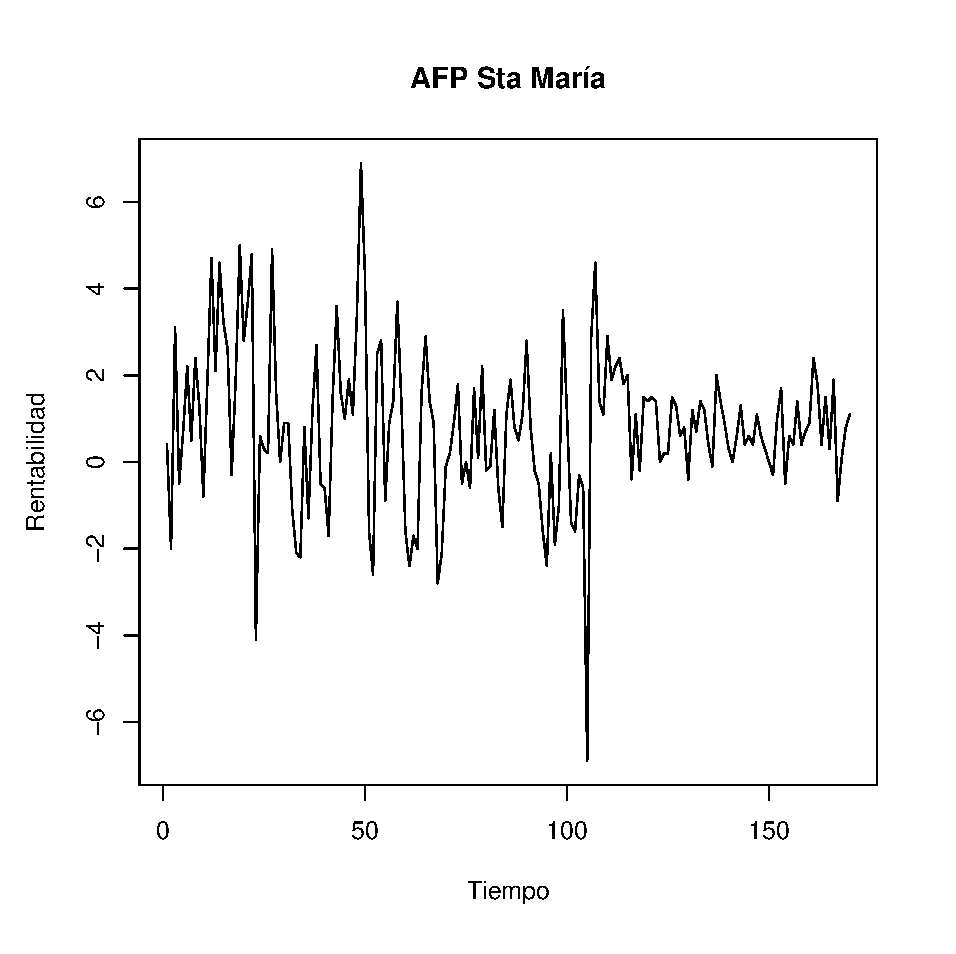
\includegraphics[height=4cm, width=4cm]{afp6.eps}
  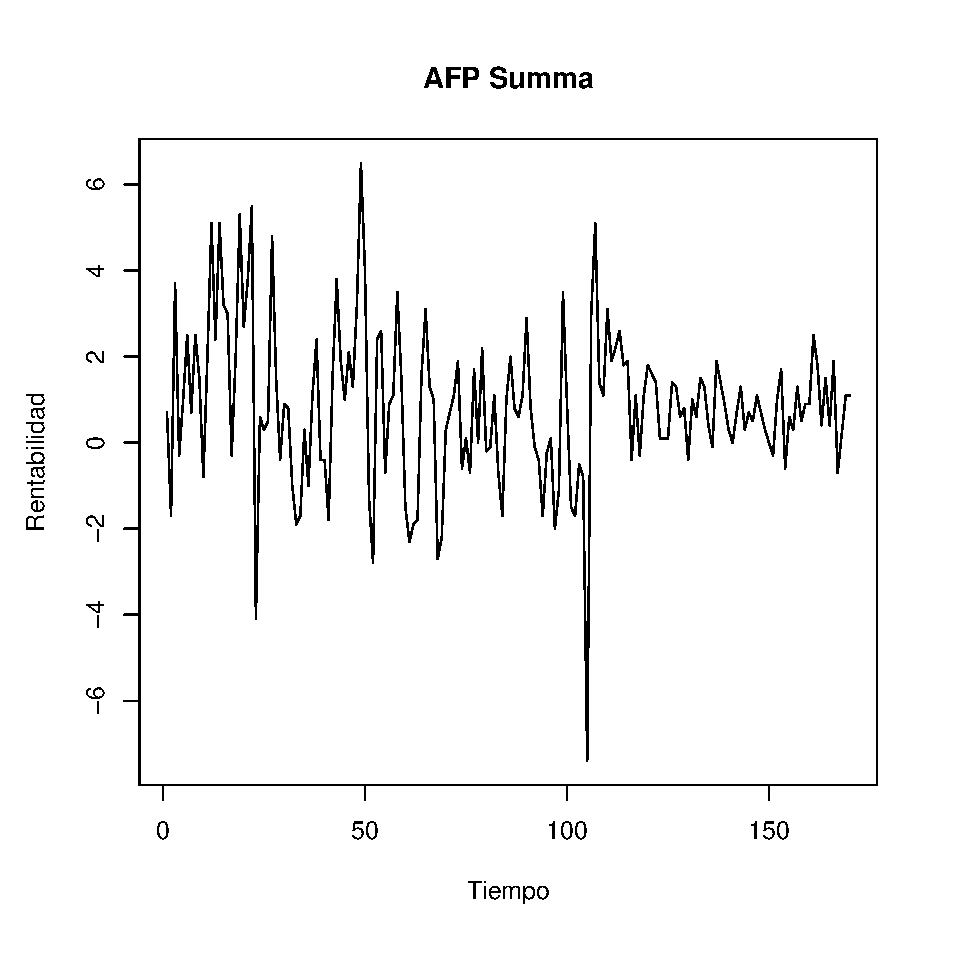
\includegraphics[height=4cm, width=4cm]{afp7.eps}
   \caption{Rentabilidad AFP.}
\label{caja}
\end{center}
\end{figure}

En estos Gr\'aficos, se puede apreciar el comportamiento similar de las 7 AFP. Donde se puede observar que en todas las AFP, en el per\'iodo de Noviembre 1997 y en Enero, Junio y Septiembre de 1998, las AFP muestran sus ca\'idas mas significativas. Con Septiembre de 1998 la ca\'ida mas importante de estas, este  dato at\'ipico podr\'ia afectar la modelaci\'on en sus par\'ametros o quiz\'as a validar el supuesto de normalidad.

Como las AFP muestran rentabilidades con valores negativos y adem\'as, se puede notar que la varianza de la rentabilidad de las AFP no es constante, proponer una tansformaci\'on que nos ayude a homogenizar la varianza y dejar las series estacionarias, se tienen que considerar estos valores. Por lo general,para homogenizar la varianza se ocupan $\sqrt(x)$ y $\log(x)$, pero como existen valores negativos, habr\'ian casos indeterminados,es por eso que se trasladara esta serie en 10 unidades, un n\'umero un poco mayor al de los valores extremos que es -7.4, para as\'i tener valores positivos y homogenizar la serie con el $\log(x)$. Acontinuaci\'on, se muestran las series transformadas:

\begin{figure}[!ht]
\begin{center}
\centering
  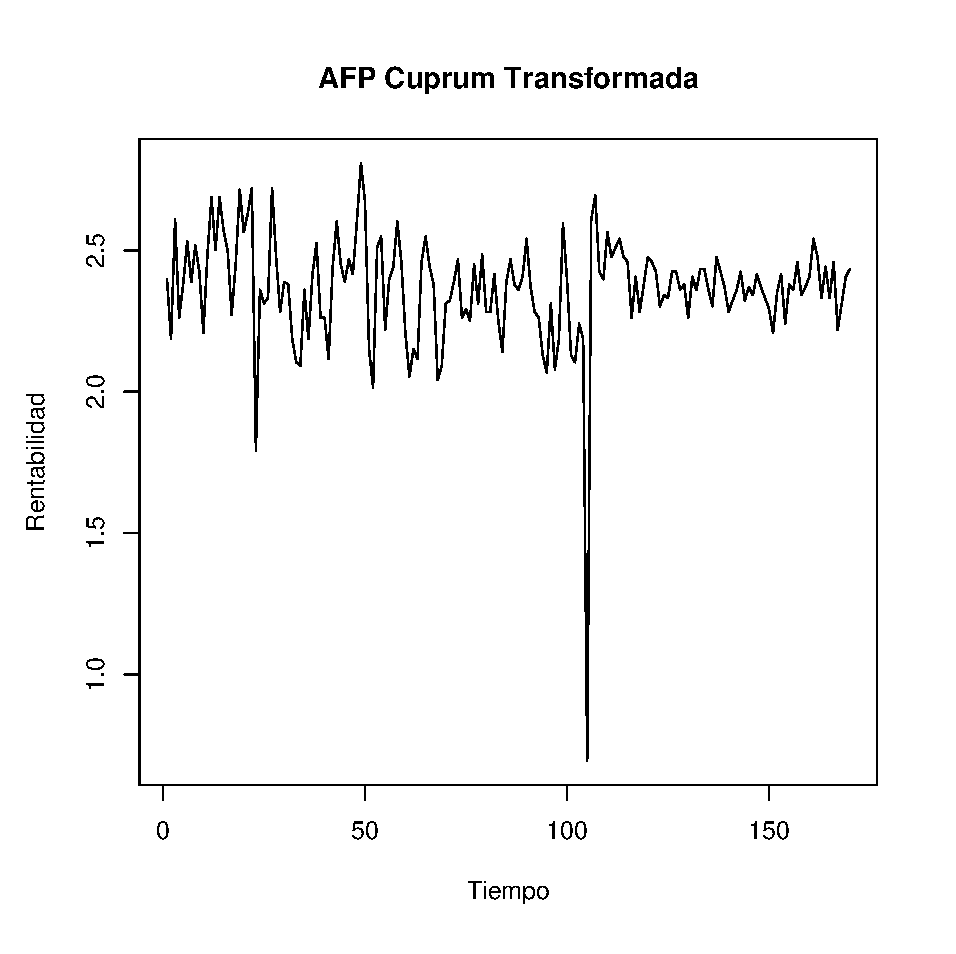
\includegraphics[height=4cm, width=4cm]{afptr1.eps}
  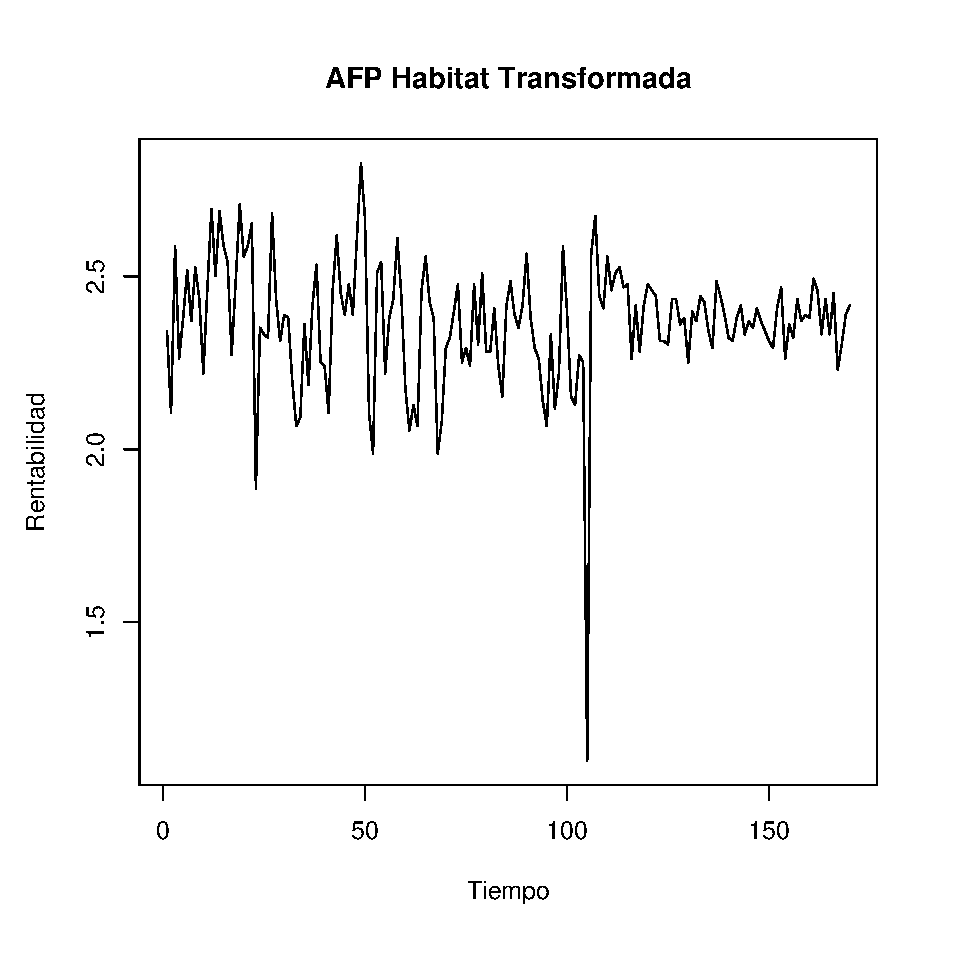
\includegraphics[height=4cm, width=4cm]{afptr2.eps}
  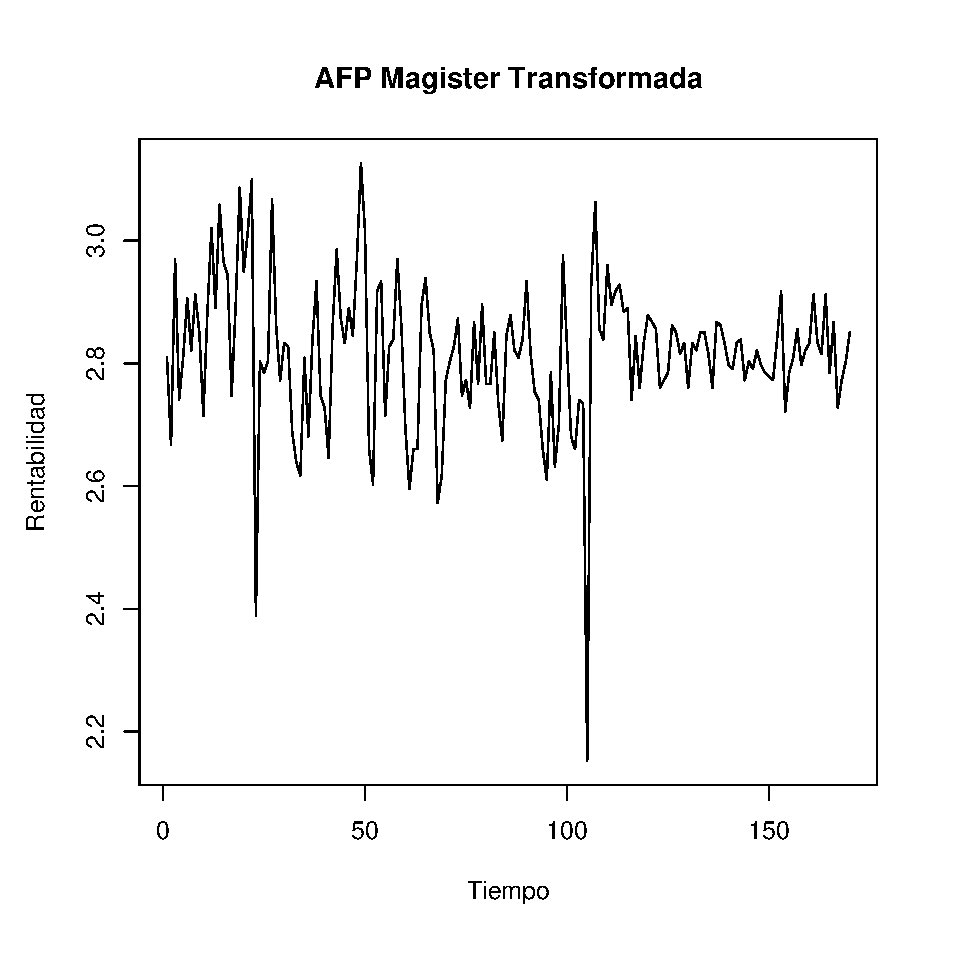
\includegraphics[height=4cm, width=4cm]{afptr3.eps}
  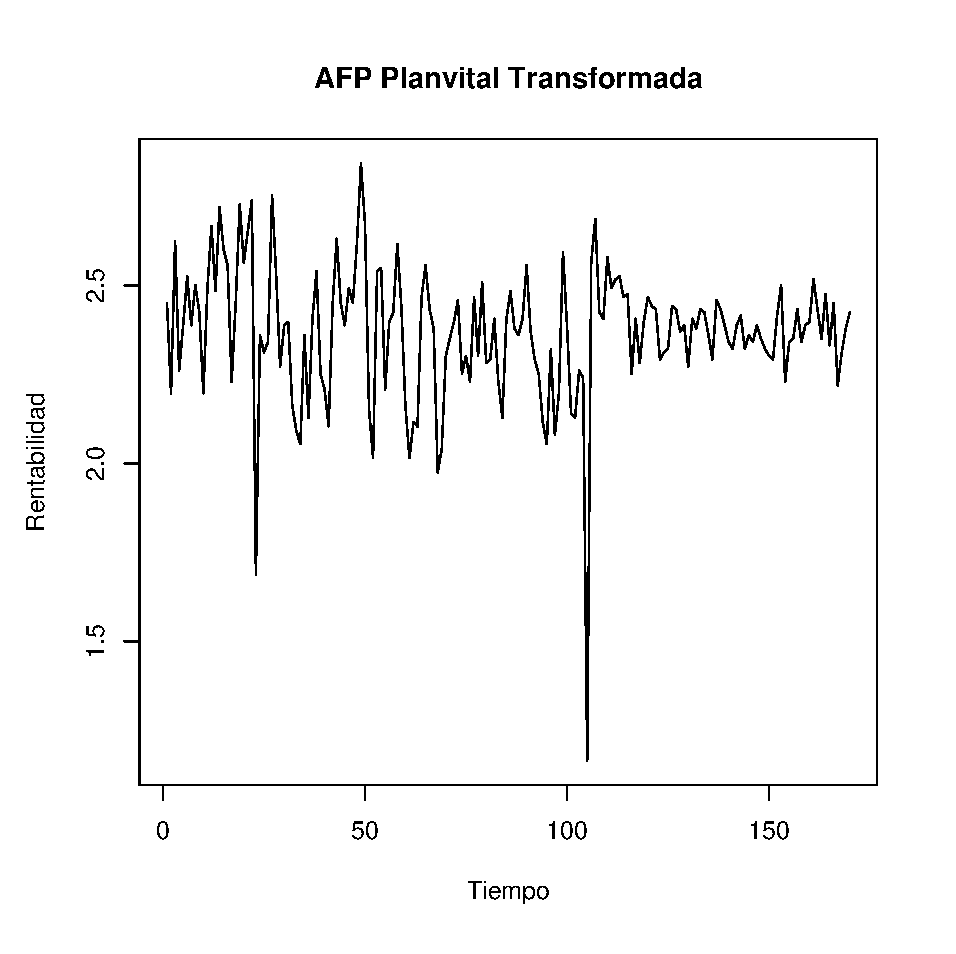
\includegraphics[height=4cm, width=4cm]{afptr4.eps}\\
  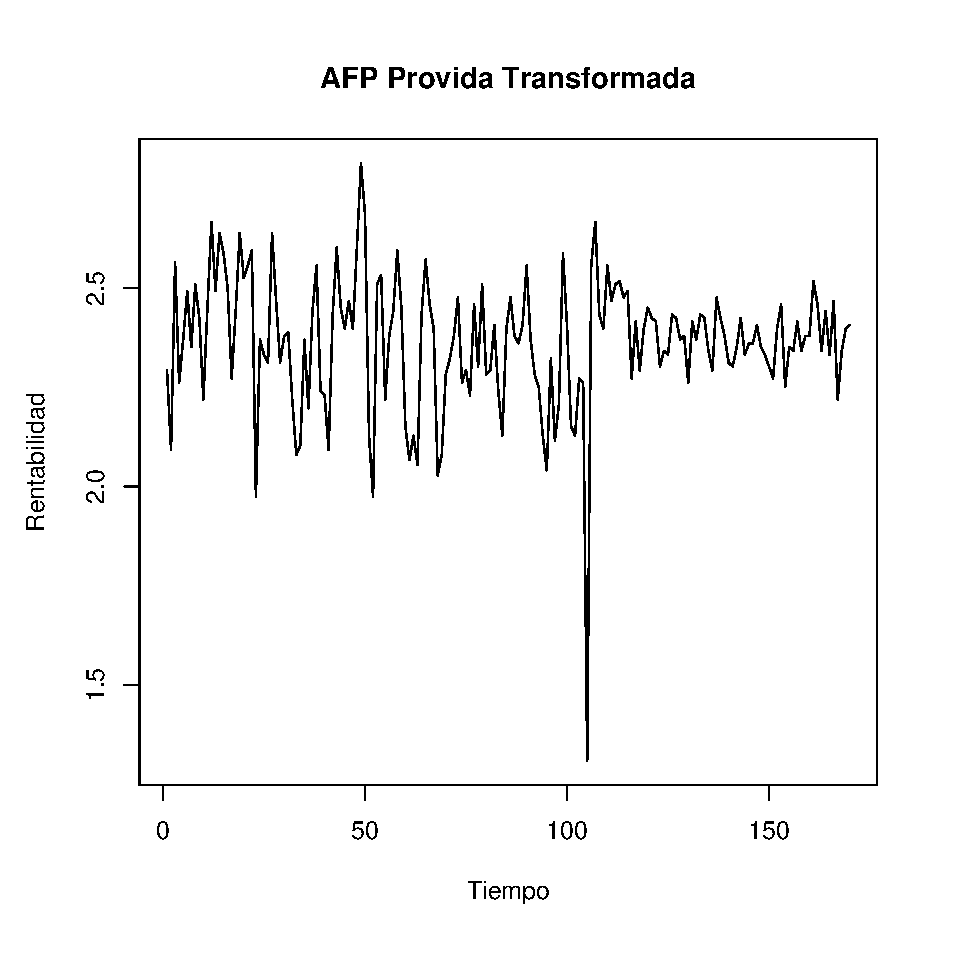
\includegraphics[height=4cm, width=4cm]{afptr5.eps}
  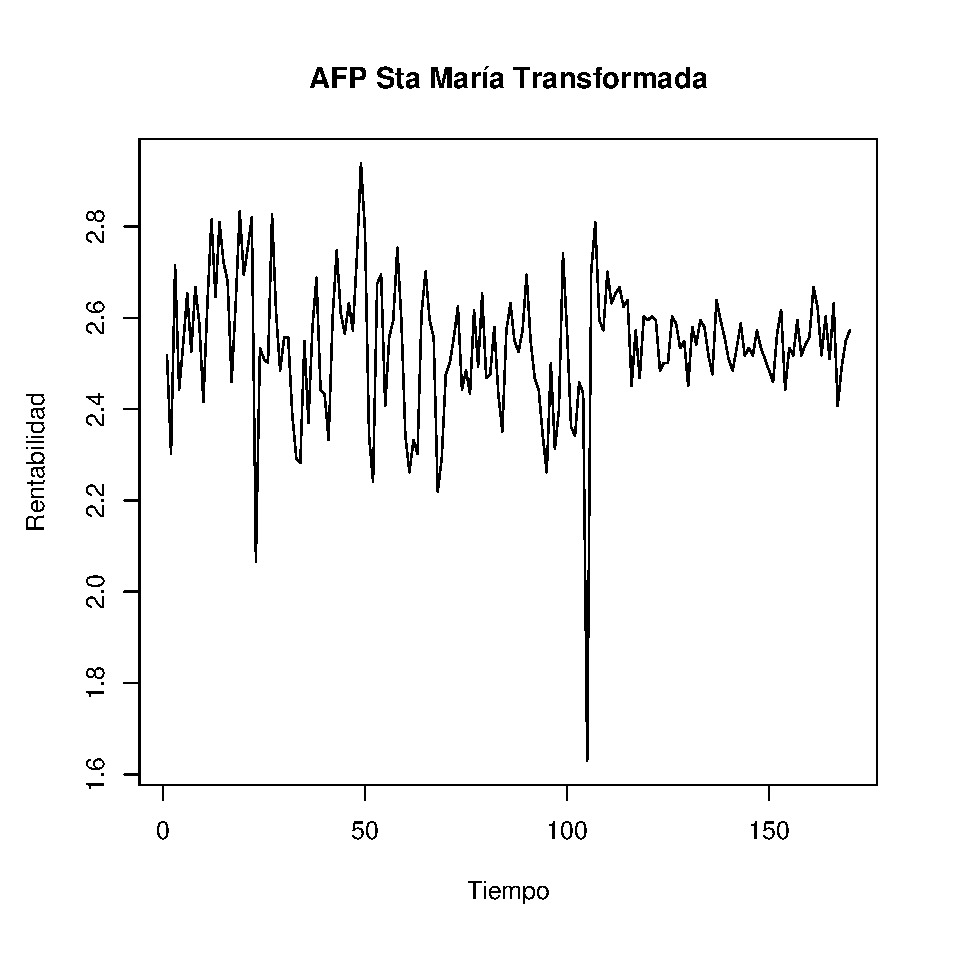
\includegraphics[height=4cm, width=4cm]{afptr6.eps}
  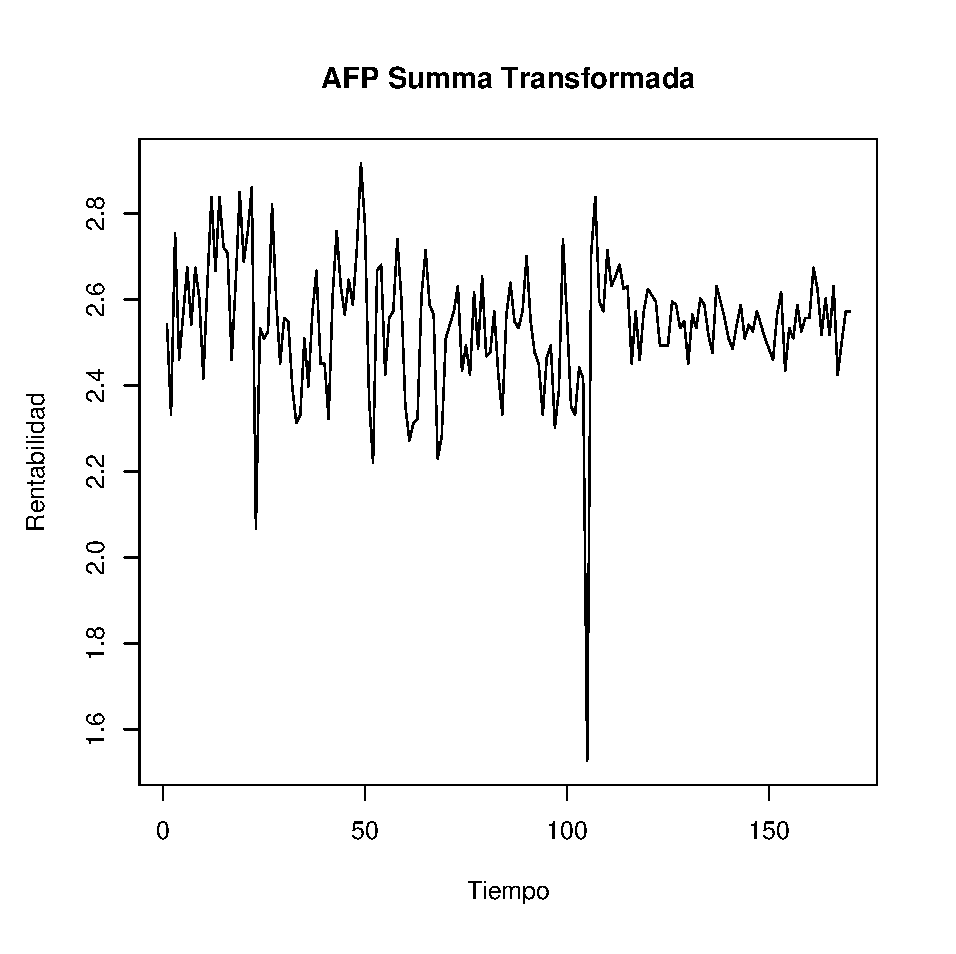
\includegraphics[height=4cm, width=4cm]{afptr7.eps}
   \caption{Transformaci\'on AFP.}
\label{caja}
\end{center}
\end{figure}

En la Figura 4.4 se puede apreciar, que si bien la serie esta m\'as estacionaria, a\'un se puede apreciar que la ca\'ida de septiembre 1998 afecta, al intentar homogenizar la varianza.

Luego de analizar la estacionariedad de las AFP, propondremos un modelo que represente esta situaci\'on. Si consideramos las funciones ACF  y Partial ACF, los resultados son los siguientes.

\begin{figure}[!ht]
\centering
  \includegraphics[height=4cm, width=4cm]{acf1.eps}
  \includegraphics[height=4cm, width=4cm]{acf2.eps}
  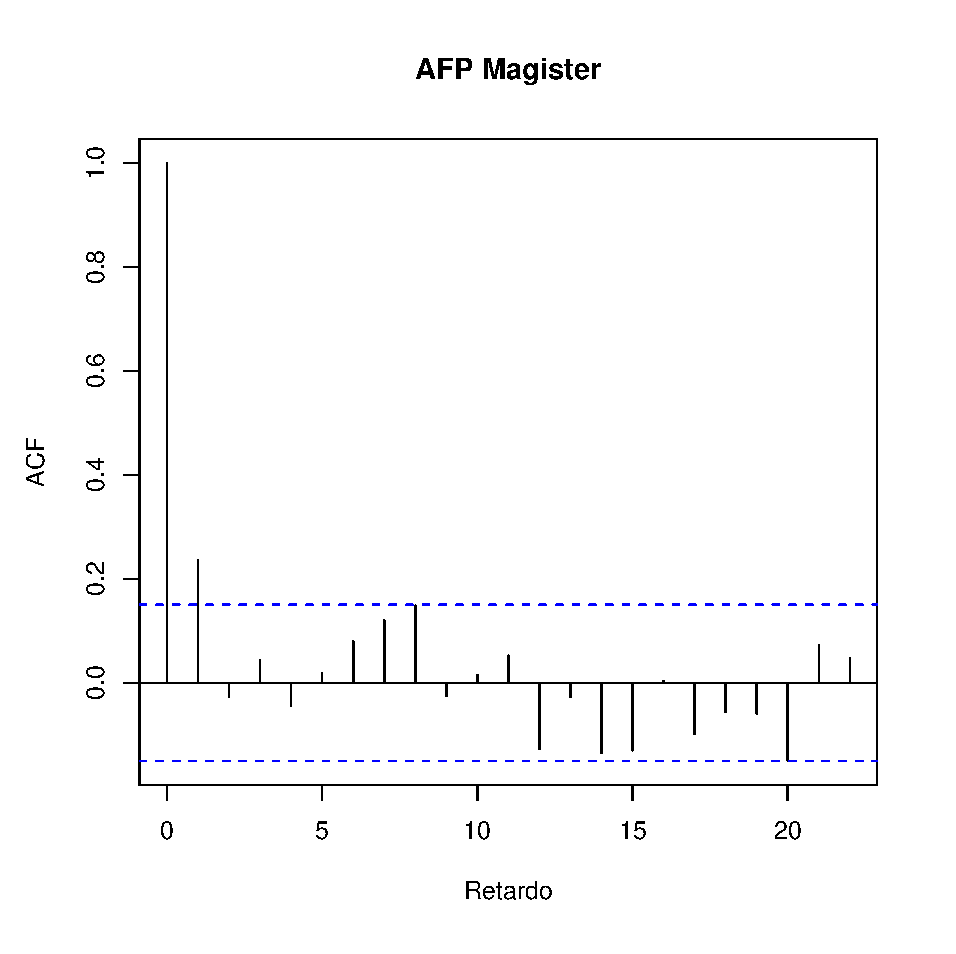
\includegraphics[height=4cm, width=4cm]{acf3.eps}
  \includegraphics[height=4cm, width=4cm]{acf4.eps}
\label{caja}
\end{figure}

\begin{figure}[!ht]
\centering
  \includegraphics[height=4cm, width=4cm]{acf5.eps}
  \includegraphics[height=4cm, width=4cm]{acf6.eps}
  \includegraphics[height=4cm, width=4cm]{acf7.eps}
   \caption{Funci\'on de Autocorrelaci\'on AFP.}
\label{caja}
\end{figure}

Se observa que la memoria del proceso  es de un retardo. Como se presento anteriormente en la Figura 4.5 de la rentabilidad de las AFP se puede observar una cierta estacionalidad, propia de los modelos de media m\'ovil. Ahora bien, se analizar\'a que sucede con la funci\'on de autocorrelaci\'on parcial

\begin{figure}[!ht]
\begin{center}
\centering
  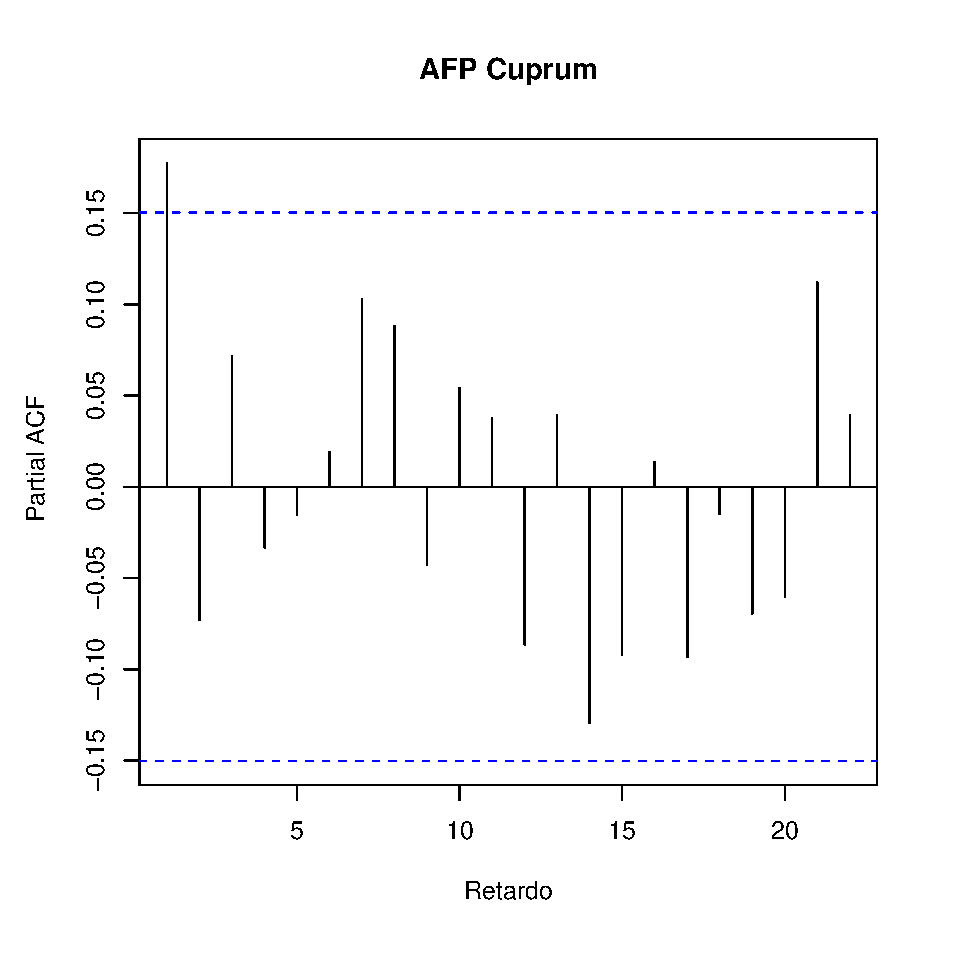
\includegraphics[height=4cm, width=4cm]{pacf1.eps}
  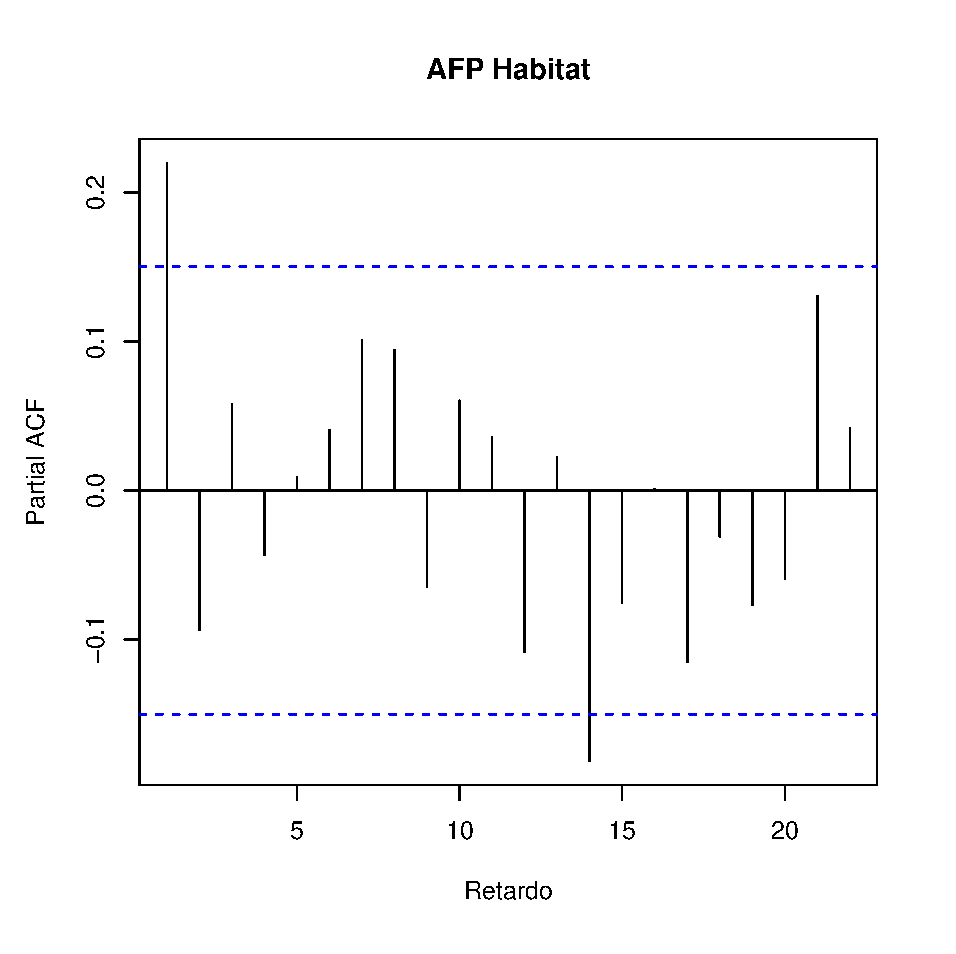
\includegraphics[height=4cm, width=4cm]{pacf2.eps}
  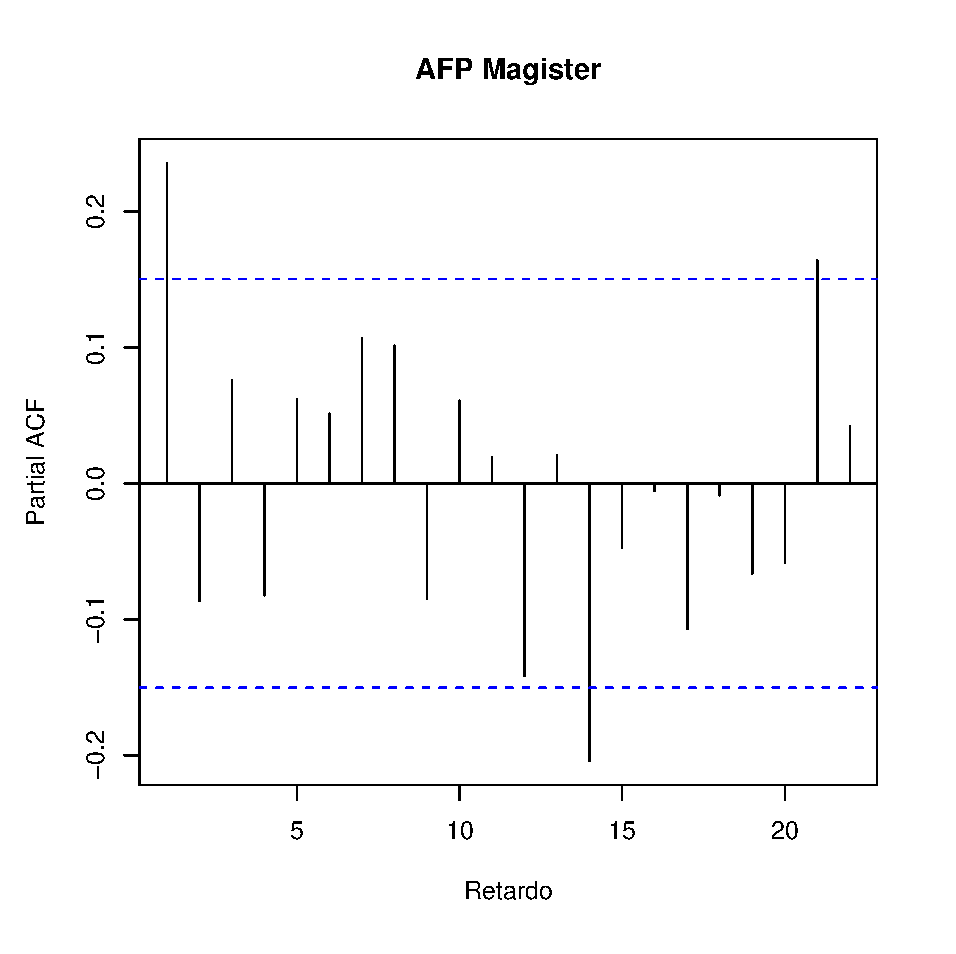
\includegraphics[height=4cm, width=4cm]{pacf3.eps}
  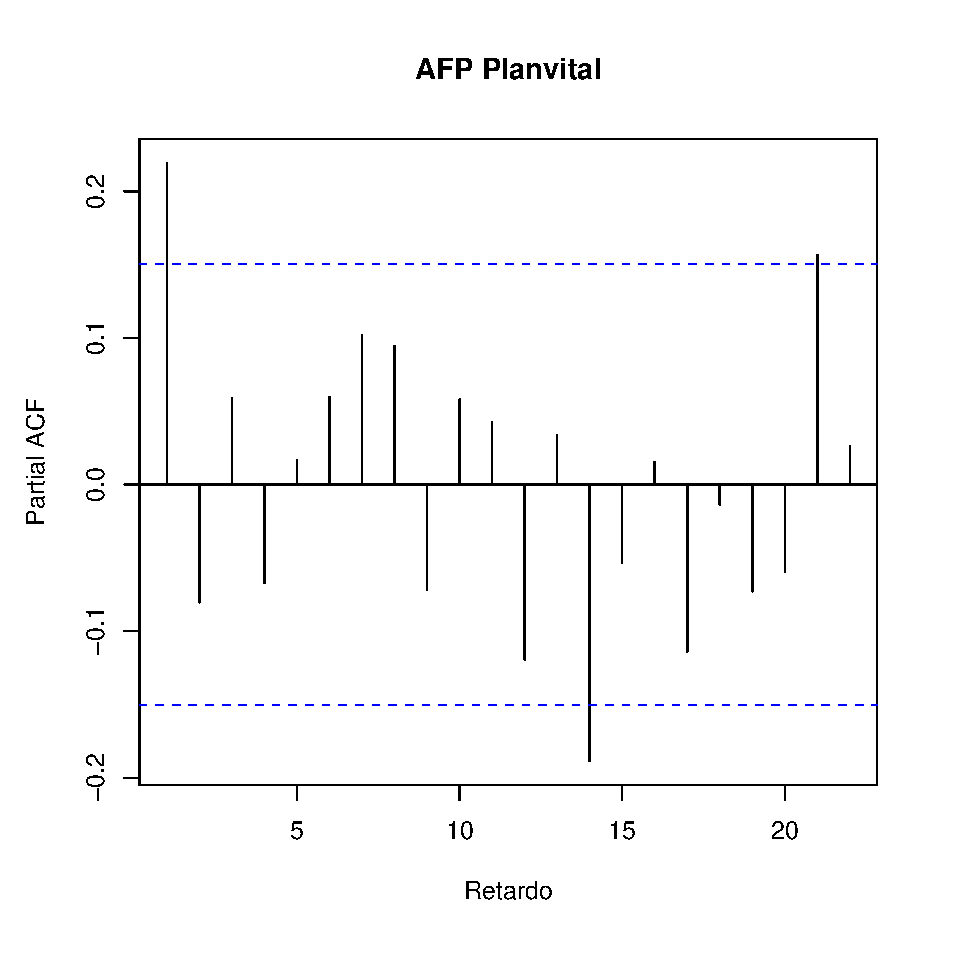
\includegraphics[height=4cm, width=4cm]{pacf4.eps}\\
  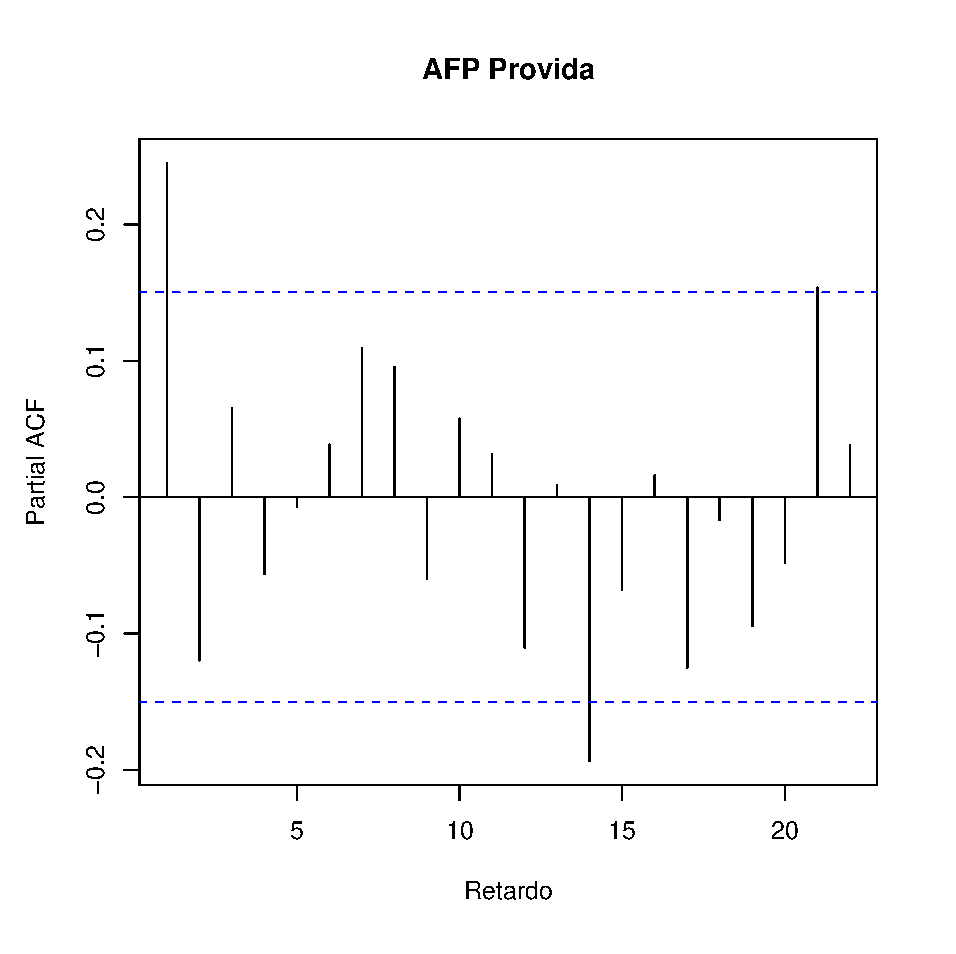
\includegraphics[height=4cm, width=4cm]{pacf5.eps}
  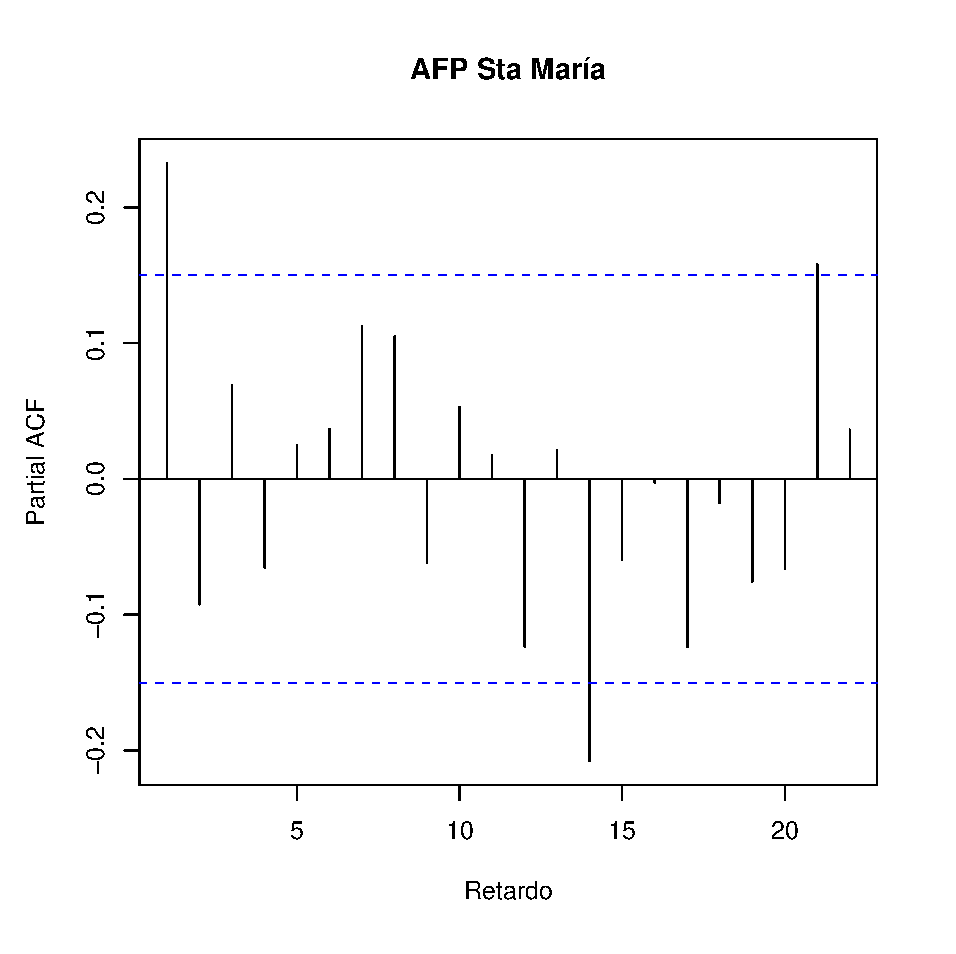
\includegraphics[height=4cm, width=4cm]{pacf6.eps}
  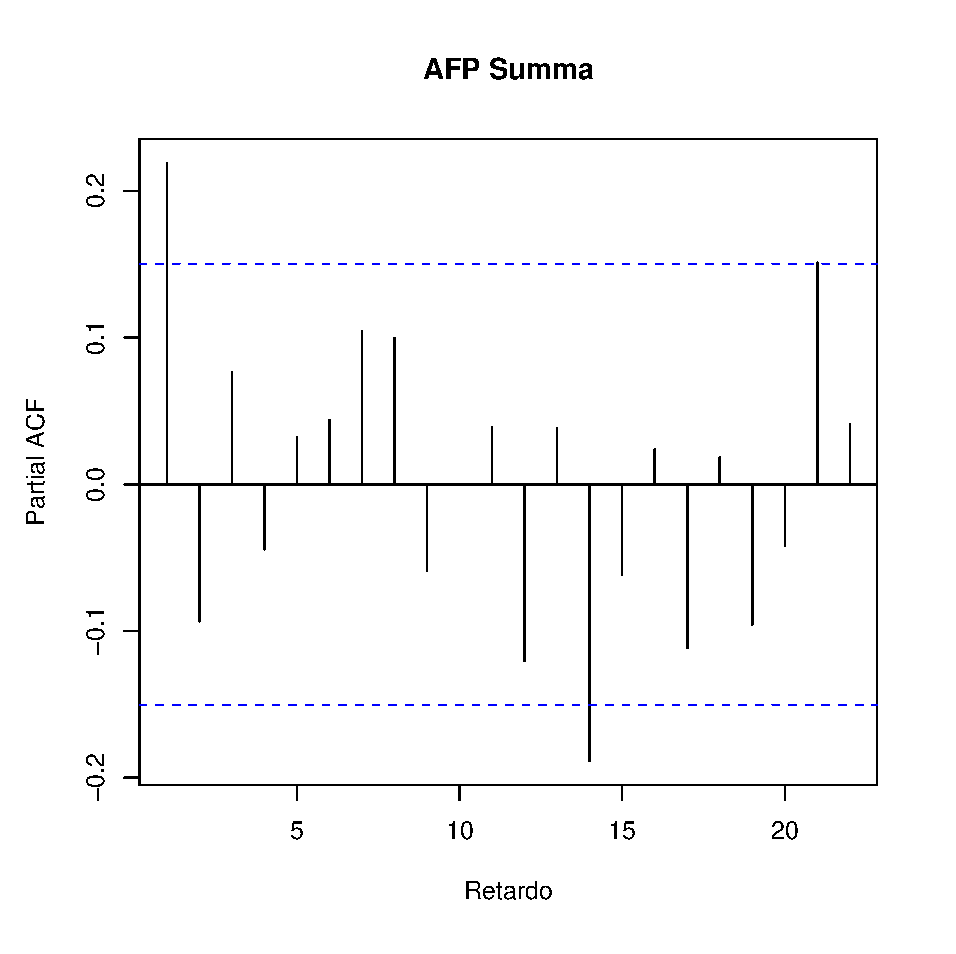
\includegraphics[height=4cm, width=4cm]{pacf7.eps}
   \caption{Funci\'on de Autocorrelaci\'on Parcial AFP.}
\label{caja}
\end{center}
\end{figure}
En base a la Figura 4.6 se pueden proponer algunos modelos a priori, para representar la rentabilidad de las AFP.\\
La parte autoregresiva contribuye en 2 lag o retardos, Por otra parte, la estructura de media mov\'il contribuye con 1 lag o retardo. Acontinuaci\'on algunas propuestas de modelos para esta situaci\'on.
\begin{center}
\begin{tabular}{|l|l|ll}
\cline{1-2}
Modelos Propuestos & AIC &  &  \\
\cline{1-2}
ARMA(1,1) & -60.71 &  &  \\
ARMA(2,1) & -58.73 &  &  \\
AR(1) & -60.98 &  &  \\
MA(1) & -61.84 &  &  \\
\cline{1-2}
\end{tabular}
\end{center}

Si se observa el AIC de los modelos propuestos, el modelo que minimiza la varianza de los residuos es el modelo de media mov\'il MA(1). Las AFP son modelados a trav\'es de  MA(1), desde aqu\'i, se puede analizar supuesto de normalidad.

\section{Estimaci\'on de par\'ametros MA(1) y an\'alisis de residuos}
En esta seccion se presentaran las estiamciones de los coeficiente de los modelos MA(1) para cada una de las AFP.
\paragraph{Estimaci\'on de par\'ametros AFP Cuprum}
\begin{center}
\begin{tabular}{|l|l|l|}
\hline
\multicolumn{1}{|c|}{Par\'ametros} & \multicolumn{1}{c|}{MA(1)} & \multicolumn{1}{c|}{Intercepto} \\
\hline
\multicolumn{1}{|c|}{Coeficiente} & \multicolumn{1}{c|}{-0,9684} & \multicolumn{1}{c|}{-1,00E-04} \\
\hline
\multicolumn{1}{|c|}{s.e} & \multicolumn{1}{c|}{0,0356} & \multicolumn{1}{c|}{3,00E-04} \\
\hline
\multicolumn{1}{|c|}{$\hat{\sigma}^{2}$} & \multicolumn{1}{c|}{Log Ver} & \multicolumn{1}{c|}{AIC} \\
\hline
\multicolumn{1}{|c|}{0,01031} & \multicolumn{1}{c|}{145,37} & \multicolumn{1}{c|}{-284,75} \\
\hline
\end{tabular}
\end{center}
\paragraph{Estimaci\'on de par\'ametros AFP Habitat}
\begin{center}
\begin{tabular}{|l|l|l|}
\hline
\multicolumn{1}{|c|}{Par\'ametros} & \multicolumn{1}{c|}{MA(1)} & \multicolumn{1}{c|}{Intercepto} \\
\hline
\multicolumn{1}{|c|}{Coeficiente} & \multicolumn{1}{c|}{-0,9675} & \multicolumn{1}{c|}{-1,00E-04} \\
\hline
\multicolumn{1}{|c|}{s.e} & \multicolumn{1}{c|}{0,0371} & \multicolumn{1}{c|}{3,00E-04} \\
\hline
\multicolumn{1}{|c|}{$\hat{\sigma}^{2}$} & \multicolumn{1}{c|}{Log Ver} & \multicolumn{1}{c|}{AIC} \\
\hline
\multicolumn{1}{|c|}{0,0084} & \multicolumn{1}{c|}{162,69} & \multicolumn{1}{c|}{-319,39} \\
\hline
\end{tabular}
\end{center}
\paragraph{Estimaci\'on de par\'ametros AFP Provida}
\begin{center}
\begin{tabular}{|l|l|l|}
\hline
\multicolumn{1}{|c|}{Par\'ametros} & \multicolumn{1}{c|}{MA(1)} & \multicolumn{1}{c|}{Intercepto} \\
\hline
\multicolumn{1}{|c|}{Coeficiente} & \multicolumn{1}{c|}{-0,9629} & \multicolumn{1}{c|}{-1,00E-04} \\
\hline
\multicolumn{1}{|c|}{s.e} & \multicolumn{1}{c|}{0,0379} & \multicolumn{1}{c|}{2,00E-04} \\
\hline
\multicolumn{1}{|c|}{$\hat{\sigma}^{2}$} & \multicolumn{1}{c|}{Log Ver} & \multicolumn{1}{c|}{AIC} \\
\hline
\multicolumn{1}{|c|}{0,003579} & \multicolumn{1}{c|}{234,85} & \multicolumn{1}{c|}{-463,71} \\
\hline
\end{tabular}
\end{center}
\paragraph{Estimaci\'on de par\'ametros AFP Planvital}
\begin{center}
\begin{tabular}{|l|l|l|}
\hline
\multicolumn{1}{|c|}{Par\'ametros} & \multicolumn{1}{c|}{MA(1)} & \multicolumn{1}{c|}{Intercepto} \\
\hline
\multicolumn{1}{|c|}{Coeficiente} & \multicolumn{1}{c|}{-0,9621} & \multicolumn{1}{c|}{-2,00E-04} \\
\hline
\multicolumn{1}{|c|}{s.e} & \multicolumn{1}{c|}{0,0346} & \multicolumn{1}{c|}{3,00E-04} \\
\hline
\multicolumn{1}{|c|}{$\hat{\sigma}^{2}$} & \multicolumn{1}{c|}{Log Ver} & \multicolumn{1}{c|}{AIC} \\
\hline
\multicolumn{1}{|c|}{0,009118} & \multicolumn{1}{c|}{155,84} & \multicolumn{1}{c|}{-305,69} \\
\hline
\end{tabular}
\end{center}
\paragraph{Estimaci\'on de par\'ametros AFP Sta. Mar\'ia}
\begin{center}
\begin{tabular}{|l|l|l|}
\hline
\multicolumn{1}{|c|}{Par\'ametros} & \multicolumn{1}{c|}{MA(1)} & \multicolumn{1}{c|}{Intercepto} \\
\hline
\multicolumn{1}{|c|}{Coeficiente} & \multicolumn{1}{c|}{-0,96} & \multicolumn{1}{c|}{4,20E-03} \\
\hline
\multicolumn{1}{|c|}{s.e} & \multicolumn{1}{c|}{0,0437} & \multicolumn{1}{c|}{6,40E-03} \\
\hline
\multicolumn{1}{|c|}{$\hat{\sigma}^{2}$} & \multicolumn{1}{c|}{Log Ver} & \multicolumn{1}{c|}{AIC} \\
\hline
\multicolumn{1}{|c|}{3,128} & \multicolumn{1}{c|}{-337,44} & \multicolumn{1}{c|}{680,88} \\
\hline
\end{tabular}
\end{center}
\paragraph{Estimaci\'on de par\'ametros AFP Summa}
\begin{center}
\begin{tabular}{|l|l|l|}
\hline
\multicolumn{1}{|c|}{Par\'ametros} & \multicolumn{1}{c|}{MA(1)} & \multicolumn{1}{c|}{Intercepto} \\
\hline
\multicolumn{1}{|c|}{Coeficiente} & \multicolumn{1}{c|}{0,2786} & \multicolumn{1}{c|}{1,27E+00} \\
\hline
\multicolumn{1}{|c|}{s.e} & \multicolumn{1}{c|}{0,0805} & \multicolumn{1}{c|}{7,10E-03} \\
\hline
\multicolumn{1}{|c|}{$\hat{\sigma}^{2}$} & \multicolumn{1}{c|}{Log Ver} & \multicolumn{1}{c|}{AIC} \\
\hline
\multicolumn{1}{|c|}{0,005291} & \multicolumn{1}{c|}{204,29} & \multicolumn{1}{c|}{-402,58} \\
\hline
\end{tabular}
\end{center}
\paragraph{Estimaci\'on de par\'ametros AFP Magister}

\begin{center}
\begin{tabular}{|l|l|l|}
\hline
\multicolumn{1}{|c|}{Par\'ametros} & \multicolumn{1}{c|}{MA(1)} & \multicolumn{1}{c|}{Intercepto} \\
\hline
\multicolumn{1}{|c|}{Coeficiente} & \multicolumn{1}{c|}{-0,9626} & \multicolumn{1}{c|}{-1,00E-04} \\
\hline
\multicolumn{1}{|c|}{s.e} & \multicolumn{1}{c|}{0,0346} & \multicolumn{1}{c|}{3,00E-04} \\
\hline
\multicolumn{1}{|c|}{$\hat{\sigma}^{2}$} & \multicolumn{1}{c|}{Log Ver} & \multicolumn{1}{c|}{AIC} \\
\hline
\multicolumn{1}{|c|}{0,005998} & \multicolumn{1}{c|}{191,22} & \multicolumn{1}{c|}{-376,44} \\
\hline
\end{tabular}
\end{center}

\paragraph{Test de bondad de ajuste}

En esta parte se presentar\'a la verificaci\'on del supuesto de normalidad de los residuos para cada modelo a trav\'es del test de Shapiro Wilks, presentando su estad\'istica y el valor-$p$.
\begin{center}
\begin{tabular}{|l|l|l|}
\hline
\multicolumn{1}{|c|}{AFP} & \multicolumn{1}{c|}{W} & \multicolumn{1}{c|}{p-valor} \\
\hline
\multicolumn{1}{|c|}{Cuprum} & \multicolumn{1}{c|}{0,7983} & \multicolumn{1}{c|}{0} \\
\hline
\multicolumn{1}{|c|}{Habitat} & \multicolumn{1}{c|}{0,8817} & \multicolumn{1}{c|}{0} \\
\hline
\multicolumn{1}{|c|}{Provida} & \multicolumn{1}{c|}{0,8946} & \multicolumn{1}{c|}{0} \\
\hline
\multicolumn{1}{|c|}{Planvital} & \multicolumn{1}{c|}{0,8924} & \multicolumn{1}{c|}{0} \\
\hline
\multicolumn{1}{|c|}{Sta. Maria} & \multicolumn{1}{c|}{0,9773} & \multicolumn{1}{c|}{0,007089} \\
\hline
\multicolumn{1}{|c|}{Summa} & \multicolumn{1}{c|}{0,9095} & \multicolumn{1}{c|}{0} \\
\hline
\multicolumn{1}{|c|}{Magister} & \multicolumn{1}{c|}{0,8946} & \multicolumn{1}{c|}{0} \\
\hline
\end{tabular}
\end{center}

A continuaci\'on se presentan histogramas de los residuos de las 7 AFP.

\begin{figure}[!htp]
\begin{center}
\centering
  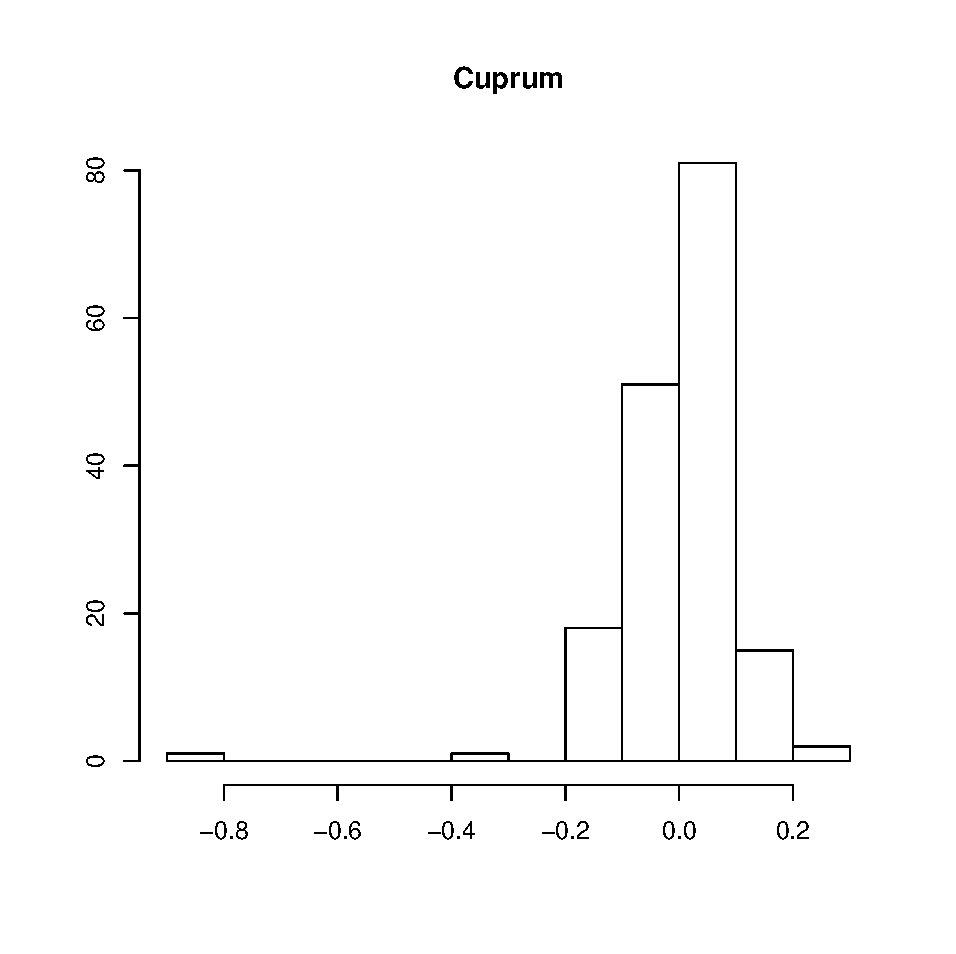
\includegraphics[height=4cm, width=4cm]{grafico1.eps}
  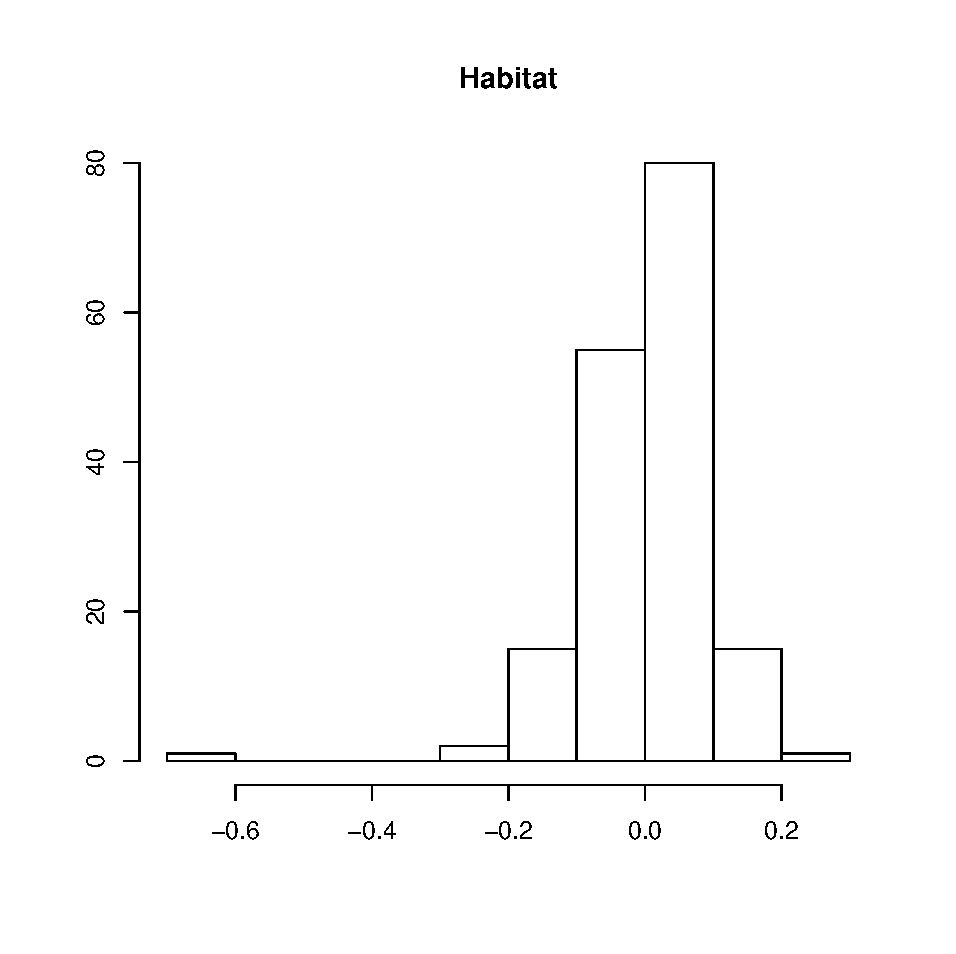
\includegraphics[height=4cm, width=4cm]{grafico2.eps}
  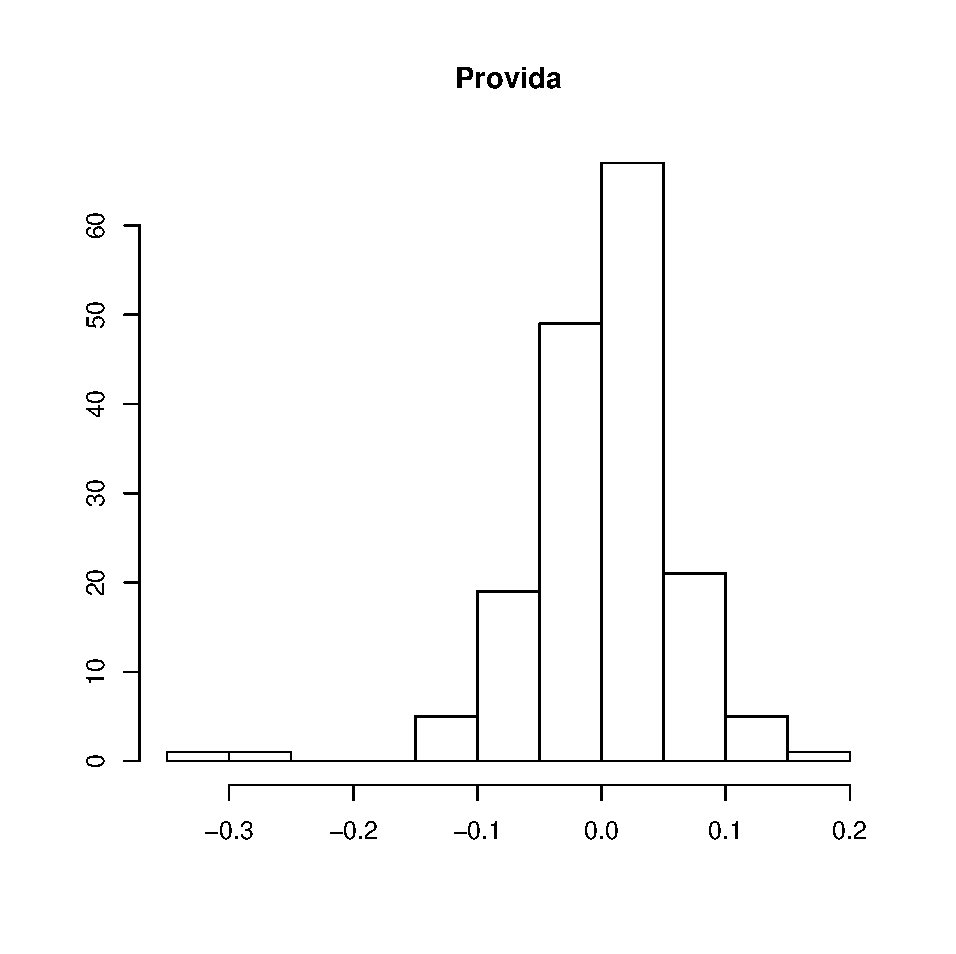
\includegraphics[height=4cm, width=4cm]{grafico3.eps}
  \includegraphics[height=4cm, width=4cm]{grafico4.eps}
  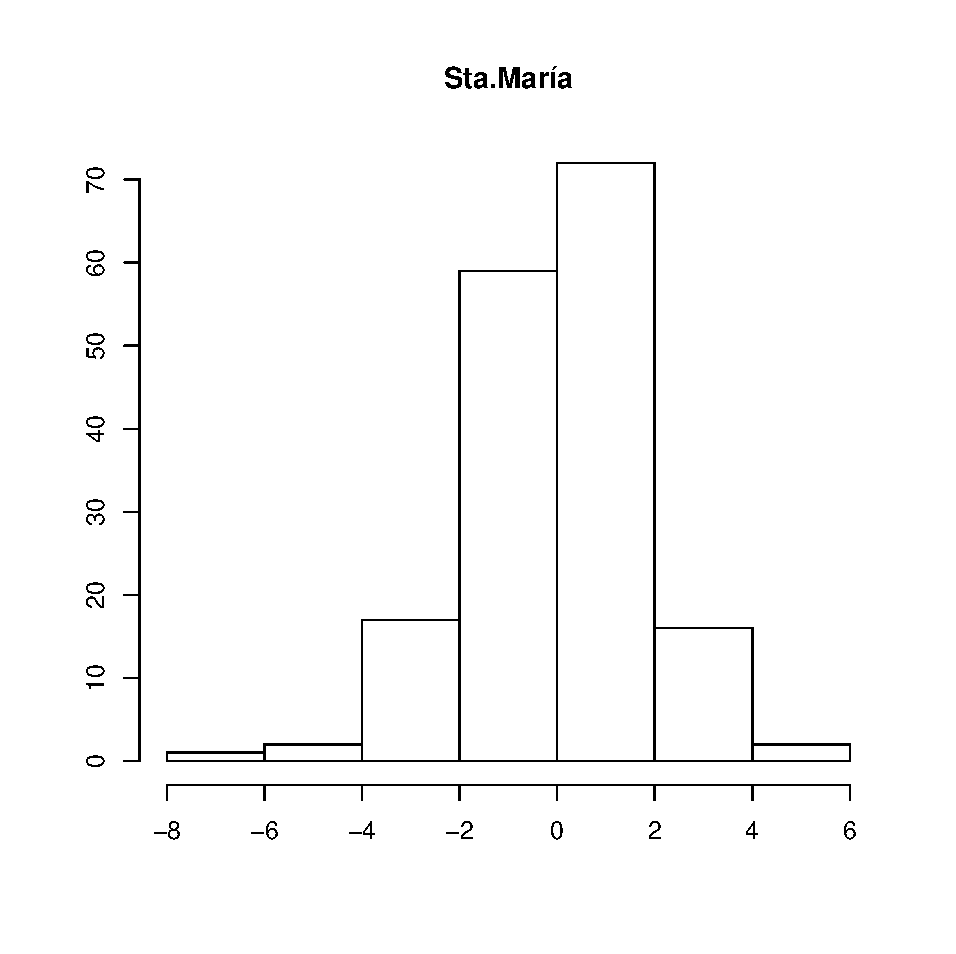
\includegraphics[height=4cm, width=4cm]{grafico5.eps}
  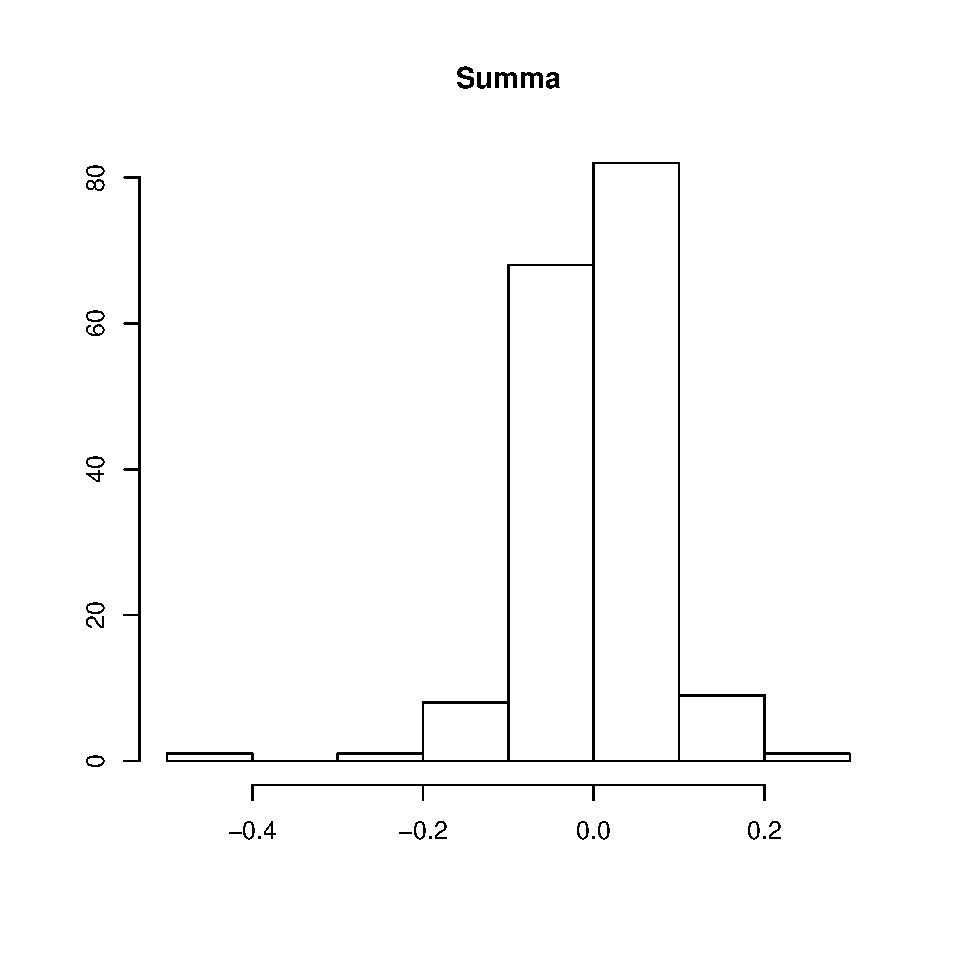
\includegraphics[height=4cm, width=4cm]{grafico6.eps}
  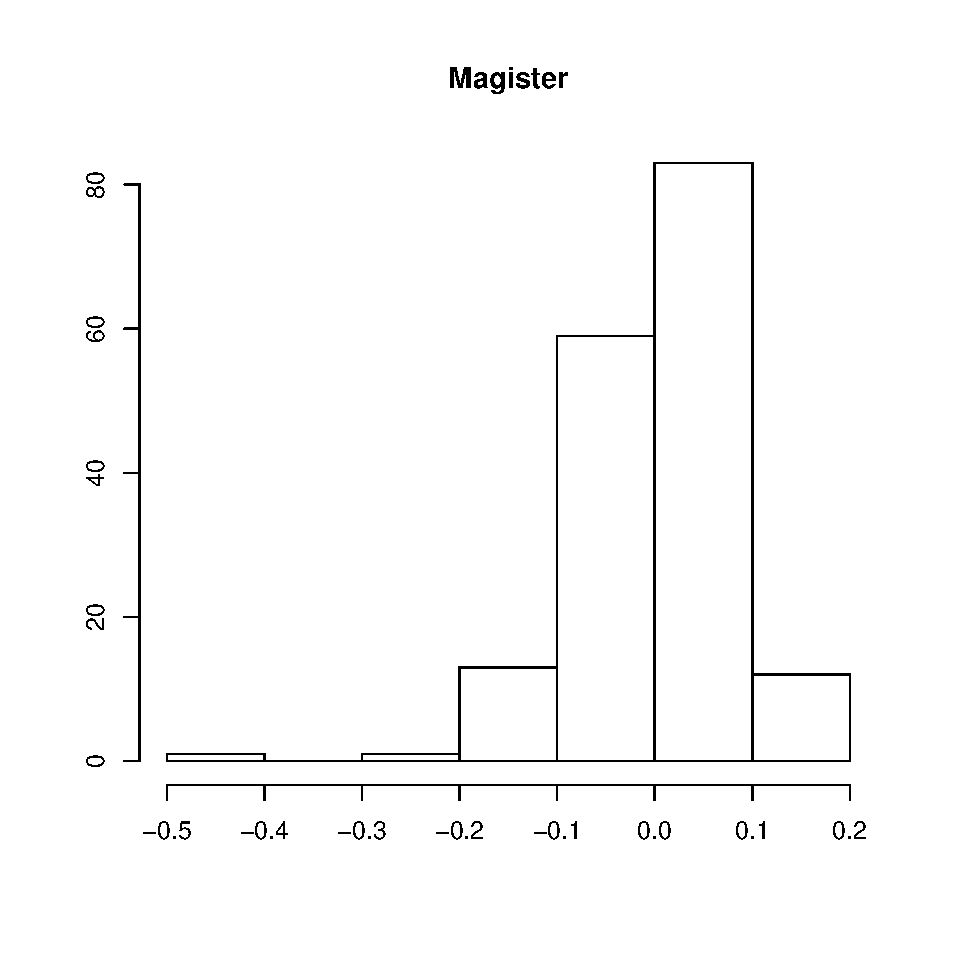
\includegraphics[height=4cm, width=4cm]{grafico7.eps}
   \caption{Histograma de los residuos AFP.}
\label{caja}
\end{center}
\end{figure}

\section{An\'alisis de Cluster}
En esta secci\'on se implementar\'a el algoritmo de clasificaci\'on para series temporales con el \'Indice de Disimilaridad Adaptativo para distancias convencionales.

Para entender mejor los dendogramas se han definido los siguientes valores que estar\'an re\-fe\-ren\-cian\-do a las AFP.

\begin{itemize}
\item 1 = AFP CUPRUM, 2 = AFP HABITAT, 3 = AFP PROVIDA, 4 = AFP PLANVITAL, 5 = AFP STA MARIA, 6 = AFP SUMMA y 7 = AFP MAGISTER
\end{itemize}

Aplicando el algoritmo de clasificaci\'on para series temporales con las distancias convencionales se tiene que:

\begin{figure}[!htp]
\begin{center}
\centering
  \includegraphics[height=4cm, width=4cm]{den_dist_euc.eps}
  \includegraphics[height=4cm, width=4cm]{den_dist_dfr.eps}
  \includegraphics[height=4cm, width=4cm]{den_dist_dtw.eps}
   \caption{Dendogramas.}
\label{caja}
\end{center}
\end{figure}

En estos gr\'aficos se puede apreciar los distintos grupos con las tres distancias:
La distancia euclidiana forma dos grupos:

\begin{tabular}{|l|l|}
\hline
Grupo 1 & Grupo 2 \\
\hline
(2)(6)(5) & (3)(4)(3)(1)(7) \\
\hline
\end{tabular}
\\
\\
La distancia de Frech\'et agrupa las AFP:

\begin{tabular}{|l|l|}
\hline
Grupo 1 & Grupo 2 \\
\hline
(3)(4)(1) & (2)(7)(5)(6) \\
\hline
\end{tabular}

La distancia DTW agrupa las AFP:

\begin{tabular}{|l|l|}
\hline
Grupo 1 & Grupo 2 \\
\hline
(3)(4) & (2)(6)(3)(1)(7) \\
\hline
\end{tabular}

\subsection{Camino Distorsionado entre AFP}
La siguiente Figura muestran la alineaci\'on entre las AFP, se presentan algunas combinaciones de la AFP CUPRUM con el resto de las AFP, y se destaca presencia de una perfecta alineaci\'on, es decir, las unidades ex\-pe\-ri\-men\-ta\-les entre par de punto son similares.

\begin{figure}[!htp]
\begin{center}
\centering
  \includegraphics[height=3cm, width=4cm]{c_d1.eps}
  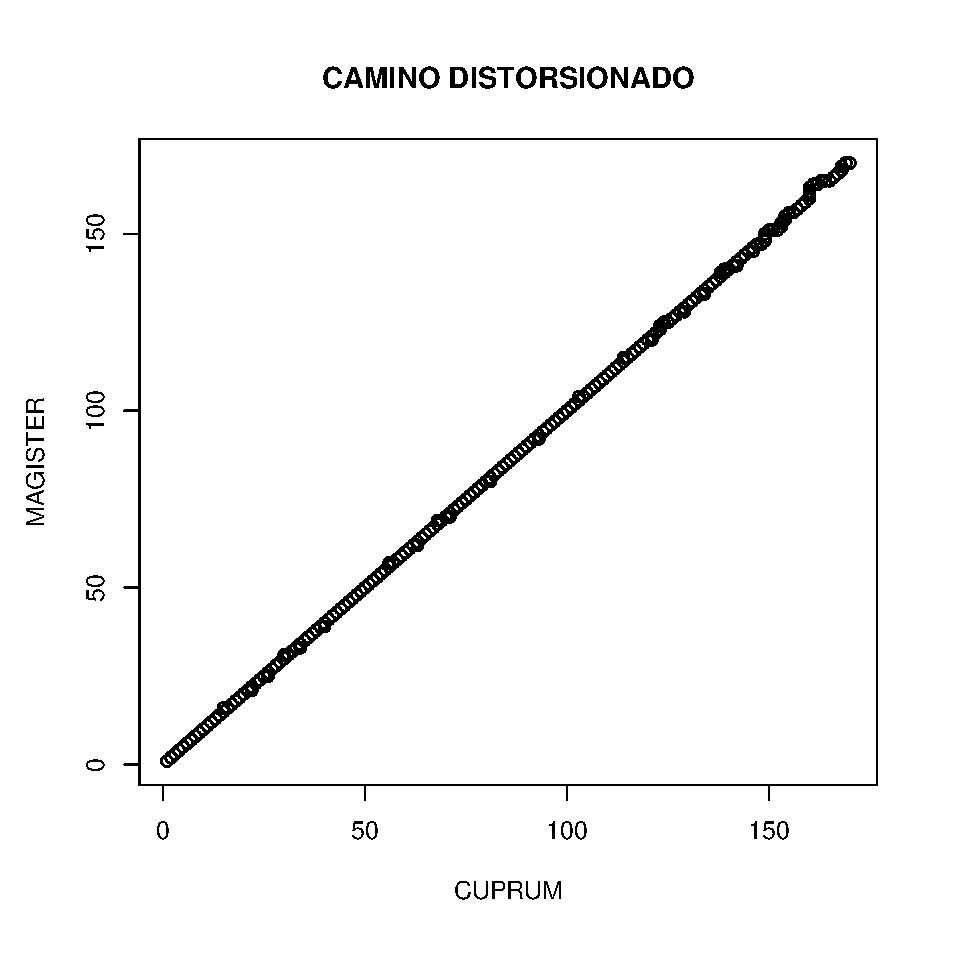
\includegraphics[height=3cm, width=4cm]{c_d2.eps}
  \includegraphics[height=3cm, width=4cm]{c_d3.eps}\\
  \includegraphics[height=3cm, width=4cm]{c_d4.eps}
  \includegraphics[height=3cm, width=4cm]{c_d5.eps}
  \includegraphics[height=3cm, width=4cm]{c_d6.eps}
   \caption{Alineamiento entre AFP.}
\label{caja}
\end{center}
\end{figure}

Esta gran similitud se debe al efecto manada, el cual ha sido detectado usando el \'Indice de Comovimiento.

\subsection{Aplicaci\'on \'Indice de Disimilaridad con Distancia Euclidiana}

Si se calcula el \'Indice usando la distancia euclidiana y se aplica el algoritmo de clasificaci\'on se puede observar que de acuerdo a la definici\'on esta calcula y re\'une las AFP que est\'an m\'as cerca respecto a cada una de las unidades experimentales, este algoritmo se calculo con $h=1,2$ y $k=1,2,3$.

\begin{figure}[!htp]
\begin{center}
\centering
  \includegraphics[height=3cm, width=4cm]{i_euc_h_1_k_1.eps}
  \includegraphics[height=3cm, width=4cm]{i_euc_h_1_k_2.eps}
  \includegraphics[height=3cm, width=4cm]{i_euc_h_1_k_3.eps}\\
  \includegraphics[height=3cm, width=4cm]{i_euc_h_2_k_1.eps}
  \includegraphics[height=3cm, width=4cm]{i_euc_h_2_k_2.eps}
  \includegraphics[height=3cm, width=4cm]{i_euc_h_2_k_3.eps}
   \caption{Dendogramas de las AFP con \'Indice usando $\delta_{E}$ con $h=1,2$ y $k=1,2,3.$}
\label{caja}
\end{center}
\end{figure}

Los dendogramas con el \'Indice Adaptativo no muestra cambios respecto de la distancia eu\-cli\-dia\-na.

\subsection{Aplicaci\'on \'Indice de Disimilaridad con Distancia Frech\'et}

Este \'Indice agrupa las AFP considerando las distancias m\'as peque\~nas dentro de las diferencias m\'aximas de cada unidad experimental. Se puede apreciar que este \'Indice presenta algunas variaciones cuando$h=2$, esta variaci\'on de agrupaci\'on es solo el intercambio de prioridad del algoritmo de Clasificaci\'on.

\begin{figure}[!htp]
\centering
  \includegraphics[height=3cm, width=4cm]{i_df_h_1_k_1.eps}
  \includegraphics[height=3cm, width=4cm]{i_df_h_1_k_2.eps}
  \includegraphics[height=3cm, width=4cm]{i_df_h_1_k_3.eps}\\
  \includegraphics[height=3cm, width=4cm]{i_df_h_2_k_1.eps}
  \includegraphics[height=3cm, width=4cm]{i_df_h_2_k_2.eps}
  \includegraphics[height=3cm, width=4cm]{i_df_h_2_k_3.eps}
  \caption{Dendogramas de las  AFP  con \'Indice usando $\delta_{F}$ con h=1,2 y k=1,2,3}
\label{caja}
\end{figure}

En general este \'Indice no presenta, cambios respecto de su distancia convencional.

\subsection{Aplicaci\'on \'Indice de Disimilaridad con Distancia DTW}

Con el \'Indice de Disimilaridad adaptativo usando la distancia $\delta_{DTW}$, agrupa las AFP que est\'an m\'as alineadas.
Este \'Indice no presenta cambios respecto de su medida convencional.

\begin{figure}[!htp]
\centering
  \includegraphics[height=3cm, width=4cm]{i_dtw_h_1_k_1.eps}
  \includegraphics[height=3cm, width=4cm]{i_dtw_h_1_k_2.eps}
  \includegraphics[height=3cm, width=4cm]{i_dtw_h_1_k_3.eps}\\
  \includegraphics[height=3cm, width=4cm]{i_dtw_h_2_k_1.eps}
  \includegraphics[height=3cm, width=4cm]{i_dtw_h_2_k_2.eps}
  \includegraphics[height=3cm, width=4cm]{i_dtw_h_2_k_3.eps}
  \caption{Dendogramas de las AFP con \'Indice usando $\delta_{DTW}$ con h=1,2 y k=1,2,3}
\label{caja}
\end{figure}
\newpage
\section{Conclusi\'on}
En este cap\'itulo se pudo conocer como se comportan las AFP, el an\'alisis descriptivo muestra evidencia de que las AFP tienen rentabilidad promedio bastante parecidas, as\'i como en la desviaci\'on est\'andar. Seguidamente, se ha propuesto un modelo que mejor representa el comportamiento de la rentabilidad, basados en la informaci\'on del AIC que son los modelos de media m\'ovil de orden 1, es decir MA(1). Adem\'as, se han calculado los par\'ametros para cada una de las 7 AFP y se analiz\'o los residuos, donde la normalidad se ve afectada fuertemente por la crisis asi\'atica en los a\~nos de 1997-1998.

En en an\'alisis de cluster, en \'Indice de Disimilaridad Adaptativo ha presentado pocos cambios respecto de sus medidas convencionales, dado la fuerte similitud de las AFP y en consecuencia, no ha podido detectar diferencias tanto en su nivel de comovimiento y de cercan\'ia.

